% !TEX encoding = UTF-8 Unicode
%
% Master thesis, print version, English.
% Class options (dyplom.cls):
%   magister / inzynier - master thesis or engineering thesis
%   druk / archiwum     - print version (for supervisor) or archive version
%   en                  - English version
%
\documentclass[magister,druk,en]{dyplom}

\usepackage[utf8]{inputenc}
\usepackage{hyperref}
\usepackage{booktabs}
\usepackage{siunitx}
\usepackage[nohyperlinks]{acronym}
\usepackage{svg}   % vector SVG figures via Inkscape (Overleaf supports it); needs --shell-escape
\svgpath{{img/}}   % search for .svg files in img/ (same folder as the other figures)

% dyplom.cls already loads microtype + fontenc (T1). As a last resort, allow a
% little extra inter-word stretch so hard paragraphs do not overrun the margin
% or leave very loose lines.
\setlength{\emergencystretch}{3em}

% TikZ is loaded by dyplom.cls; load the libraries needed for the flow diagrams.
\usetikzlibrary{arrows.meta, positioning, shapes.geometric}

% Look for figures in the local img/ folder (copied from results/.../figures).
\graphicspath{{img/}}

% Numbering depth: chapter.section.subsection (three layers max, per
% supervisor feedback 2026-06-13). Deeper levels (subsubsection, paragraph)
% render as unnumbered run-in headings.
\setcounter{secnumdepth}{2}

% ---- Title-page metadata -------------------------------------------------
\fieldofstudy{Advanced Computer Science}
\author{Sevda Aksünger}
\title{Machine-Learning-Based Framework to Monitor Handover Performance in 5G Networks}
\supervisor{dr inż. Aleksandra Knapińska}
% \consultant{Consultant's name}            % Uncomment if applicable
% \specialisation{AAA}                      % Uncomment if applicable
\keywords{handover optimization, anomaly detection, concept drift, network monitoring, 5G/6G}
% --------------------------------------------------------------------------

\begin{document}

\maketitle

\abstract{
% English abstract.

Handover (HO) management is one of the most important mobility functions in
fifth-generation (5G) and emerging sixth-generation (6G) radio access networks. When handovers are configured or monitored
poorly they cause radio link failures (RLF), ping-pong effects, and a worse
experience for the user, and as networks become denser every user goes through
many more of them, which makes reliable HO monitoring increasingly important.
This thesis studies one question in particular: does HO monitoring become more
reliable when short-term anomalies and long-term concept drift are handled
together instead of separately? The work is scoped to intra-RAT, inter-gNB
handover in 5G Standalone (SA) networks, meaning handover between cells that use
the same radio access technology (RAT) but are served by different base stations
(next-generation NodeBs, gNBs). This is among the most common mobility
situations in dense deployments.

A practical obstacle shapes the methodology. No public dataset exposes the HO
control parameters (time-to-trigger, hysteresis, A3 offset) together with the
mobility key performance indicators (KPIs) they produce, so the main data comes
from a custom 5G New Radio (NR) SA handover simulator built to follow the
relevant 3rd Generation Partnership Project (3GPP) procedures. Its radio layer is calibrated against the real NordicDat drive-test
data, with close agreement for reference signal received power (RSRP) and
signal-to-interference-plus-noise ratio (SINR) and a documented residual
mismatch for reference signal received quality (RSRQ). Real and simulated
samples are never mixed, so the benchmark stays clean.

On this data the thesis builds and compares four layers: unsupervised anomaly
detection on HO KPI windows, concept-drift detection on KPI streams, a
drift-aware monitor that retrains the anomaly detector when drift is detected,
and a configuration-performance surrogate that links HO parameters to mobility
outcomes.

Four findings stand out. Unsupervised detectors catch structured faults well,
with the area under the precision--recall curve (PR-AUC) reaching $0.858$, but
miss most subtle ones. Every injected drift is
eventually detected, so the real design choice is a trade-off between detection
latency and false alarms rather than whether drift is seen at all. Retraining the
monitor naively on recent data backfires: it absorbs post-drift anomalies into
``normal'' and roughly halves detection quality, a self-poisoning effect. A
simple self-supervised filter that drops the most suspicious windows before
retraining repairs this and more than triples drift-phase PR-AUC. Finally, a
gradient-boosting surrogate predicts the handover success rate (HOSR) accurately
($R^2 = 0.96$) and, wrapped
in conformal prediction intervals, drives an end-to-end detect, recommend, and
recover loop with a model-predicted HOSR gain of $+0.62$. The overall message is
that how a monitor is kept up to date matters more than whether it is updated at
all.

}{
% Streszczenie w języku polskim.

Zarządzanie przełączeniem (handover, HO) jest jedną z najważniejszych funkcji
mobilności w sieciach radiowych piątej generacji (5G) oraz powstających
sieciach szóstej generacji (6G). Źle
skonfigurowane lub źle monitorowane przełączenia powodują utratę połączenia
radiowego (radio link failure, RLF), efekt ping-pong i pogorszenie jakości użytkowania, a wraz z
zagęszczaniem sieci każdy użytkownik wykonuje ich znacznie więcej, co czyni
niezawodne monitorowanie HO coraz ważniejszym. Praca bada jedno pytanie: czy
monitorowanie HO staje się bardziej niezawodne, gdy krótkoterminowe anomalie i
długoterminowy dryf pojęć są traktowane łącznie, a nie osobno. Zakres ograniczono
do przełączeń intra-RAT, inter-gNB w sieciach 5G w trybie Standalone (SA), czyli
przełączeń między komórkami korzystającymi z tej samej technologii dostępu
radiowego (radio access technology, RAT), lecz obsługiwanymi przez różne stacje
bazowe (next-generation NodeB, gNB). Jest to jeden z najczęstszych scenariuszy
mobilności w gęstych sieciach.

Metodologię kształtuje praktyczne ograniczenie. Żaden publiczny zbiór danych nie
udostępnia jednocześnie parametrów sterujących HO (time-to-trigger, histereza,
offset A3) oraz wynikających z nich kluczowych wskaźników wydajności (key
performance indicators, KPI) mobilności, dlatego główne dane pochodzą z własnego
symulatora przełączeń 5G New Radio (NR) SA, zbudowanego zgodnie z odpowiednimi
procedurami organizacji 3rd Generation Partnership Project (3GPP). Jego warstwę radiową skalibrowano względem
rzeczywistych danych z testów drogowych NordicDat, z dobrą zgodnością dla mocy
odbieranego sygnału referencyjnego (reference signal received power, RSRP) i
stosunku sygnału do interferencji i szumu (signal-to-interference-plus-noise
ratio, SINR) oraz udokumentowaną resztkową rozbieżnością dla jakości odbieranego
sygnału referencyjnego (reference signal received quality, RSRQ). Danych
rzeczywistych
nigdy nie łączono z symulowanymi, dzięki czemu benchmark pozostaje czysty.

Na tych danych zbudowano i porównano cztery warstwy: nienadzorowaną detekcję
anomalii w oknach KPI przełączeń, detekcję dryfu pojęć w strumieniach KPI,
monitor świadomy dryfu, który ponownie uczy detektor anomalii po wykryciu
dryfu, oraz zastępczy model konfiguracja--wydajność łączący parametry HO z
wynikami mobilności.

Wyróżniają się cztery wyniki. Detektory nienadzorowane dobrze wykrywają usterki
strukturalne, z polem pod krzywą precyzja--czułość (PR-AUC) sięgającym $0,858$,
lecz w większości pomijają subtelne. Każdy
wstrzyknięty dryf zostaje ostatecznie wykryty, więc rzeczywistym wyborem
projektowym jest kompromis między opóźnieniem detekcji a fałszywymi alarmami, a
nie to, czy dryf w ogóle zostanie zauważony. Naiwne ponowne uczenie monitora na
bieżących danych przynosi efekt odwrotny: wchłania anomalie po dryfie do
``normy'' i w przybliżeniu o połowę obniża jakość detekcji, co jest efektem
samozatrucia. Prosty samonadzorowany filtr, który usuwa najbardziej podejrzane
okna przed ponownym uczeniem, naprawia to i ponad trzykrotnie zwiększa PR-AUC w
fazie dryfu. Wreszcie zastępczy model oparty na gradient boosting trafnie
przewiduje współczynnik skuteczności przełączeń (HOSR) z $R^2 = 0,96$ i,
opakowany w konformalne przedziały predykcji,
napędza kompletną pętlę: wykryj, rekomenduj, przywróć, z przewidzianym przez
model wzrostem HOSR o $+0,62$. Ogólny wniosek jest taki, że sposób aktualizowania
monitora ma większe znaczenie niż to, czy jest on w ogóle aktualizowany.

}


\tableofcontents

% !TEX encoding = UTF-8 Unicode
% !TEX root = thesis.tex
%
% List of acronyms used in the thesis. Rendered with the `acronym` package.
% The widest short form is given in [..] after \begin{acronym} for alignment.
% Each entry: \acro{cleankey}[DISPLAY]{Full expansion}.

\chapter*{List of Acronyms}

\begin{acronym}[ROC--AUC]
  \acro{TGPP}[3GPP]{3rd Generation Partnership Project}
  \acro{ADWIN}[ADWIN]{Adaptive Windowing}
  \acro{AI}[AI]{Artificial Intelligence}
  \acro{AMF}[AMF]{Access and Mobility Management Function}
  \acro{CHO}[CHO]{Conditional Handover}
  \acro{CIO}[CIO]{Cell Individual Offset}
  \acro{DAPS}[DAPS]{Dual Active Protocol Stack}
  \acro{DDM}[DDM]{Drift Detection Method}
  \acro{DRL}[DRL]{Deep Reinforcement Learning}
  \acro{EDDM}[EDDM]{Early Drift Detection Method}
  \acro{gNB}[gNB]{next-generation Node B}
  \acro{GNN}[GNN]{Graph Neural Network}
  \acro{HO}[HO]{Handover}
  \acro{KPI}[KPI]{Key Performance Indicator}
  \acro{KS}[KS]{Kolmogorov--Smirnov}
  \acro{KSWIN}[KSWIN]{Kolmogorov--Smirnov Windowing}
  \acro{LOF}[LOF]{Local Outlier Factor}
  \acro{LTE}[LTE]{Long-Term Evolution}
  \acro{ML}[ML]{Machine Learning}
  \acro{MMD}[MMD]{Maximum Mean Discrepancy}
  \acro{MRO}[MRO]{Mobility Robustness Optimization}
  \acro{NR}[NR]{New Radio}
  \acro{NSA}[NSA]{Non-Standalone}
  \acro{OCSVM}[OC-SVM]{One-Class Support Vector Machine}
  \acro{ORAN}[O-RAN]{Open Radio Access Network}
  \acro{PCA}[PCA]{Principal Component Analysis}
  \acro{PPO}[PPO]{Proximal Policy Optimization}
  \acro{PRAUC}[PR--AUC]{Precision--Recall Area Under the Curve}
  \acro{RAN}[RAN]{Radio Access Network}
  \acro{RAT}[RAT]{Radio Access Technology}
  \acro{RIC}[RIC]{RAN Intelligent Controller}
  \acro{RLF}[RLF]{Radio Link Failure}
  \acro{ROCAUC}[ROC--AUC]{Receiver Operating Characteristic Area Under the Curve}
  \acro{RRC}[RRC]{Radio Resource Control}
  \acro{RSRP}[RSRP]{Reference Signal Received Power}
  \acro{RSRQ}[RSRQ]{Reference Signal Received Quality}
  \acro{RSSI}[RSSI]{Received Signal Strength Indicator}
  \acro{SA}[SA]{Standalone}
  \acro{SINR}[SINR]{Signal-to-Interference-plus-Noise Ratio}
  \acro{SON}[SON]{Self-Organizing Network}
  \acro{SVM}[SVM]{Support Vector Machine}
  \acro{TTT}[TTT]{Time-to-Trigger}
  \acro{UE}[UE]{User Equipment}
  \acro{UPF}[UPF]{User Plane Function}
\end{acronym}


\chapter{Introduction}
\label{ch:intro}

Every time a moving user crosses a cell border, the network must hand the radio connection over to the next cell without dropping it. This handover (HO) process is one of the key control functions in cellular communication systems, and it is under growing pressure: 5G and future radio access networks (RANs) pack more users into denser small cells at higher carrier frequencies, so the radio environment changes faster and each user performs more handovers~\cite{hoMgmtSurvey2025}. An incorrectly configured or poorly monitored handover can lead to HO failures, ping-pong effects, or radio link failures (RLF) that directly degrade the quality of service experienced by the user equipment (UE)~\cite{tr36839}. Reliable handover monitoring is therefore becoming a central concern in modern mobile networks.

However, HO-related KPI degradations are not all of the same kind. Some appear as short-term local anomalies, often caused by transient or hard-to-observe events in the network~\cite{chandola2009anomaly}. Others stem from longer-term changes in network behavior, where the statistical properties of the data evolve over time---a phenomenon commonly termed \emph{concept drift}~\cite{gama2014survey,lu2018drift}, which can make monitoring or prediction models gradually lose accuracy as conditions change. Anomaly detection targets unusual short-term behavior, whereas concept drift detection recognizes changes in what should count as normal. The two are closely linked and need to be analyzed together: otherwise transient disruptions are easily confused with long-term model degradation, leading to incorrect monitoring decisions and unreliable optimisation actions.

This thesis focuses specifically on the intra-RAT inter-gNB HO scenario, that is, a handover between cells that belong to different base stations (gNBs) but use the same radio access technology. In a dense 5G deployment neighbouring cells typically belong to different gNBs, which makes this the everyday, operationally important mobility case. Compared to inter-RAT transitions, intra-RAT handovers also offer a more homogeneous technical environment for the analysis pursued here~\cite{ts38300,ts37340}. The scenario is thus both practically important and tractable as a research target.

AI-based HO prediction and optimization have already been studied extensively~\cite{seq2seqMob2022,slicedDRL2024}, anomaly detection on cellular and O-RAN performance metrics is itself an active research area~\cite{oranAnomaly2025,oranBenchmark2023}, and concept drift detection and KPI forecasting are receiving growing attention in mobile-network monitoring~\cite{leaf,forecast5g2024}. These directions, however, are usually pursued separately: a unified HO monitoring framework that jointly handles anomaly detection, concept drift detection, and configuration--performance analysis for intra-RAT inter-gNB scenarios remains largely missing. This gap is the main motivation for the thesis, which investigates how HO behavior in 5G/6G RANs can be monitored more reliably by separating short-term anomalies from long-term behavioral changes and analyzing how these changes interact with the HO configuration parameters.

\section{The aim and scope of the thesis}

The main objective of this thesis is to develop a framework for adaptive HO monitoring under changing network conditions, combining anomaly detection, concept drift detection, drift-aware model maintenance, and configuration--performance modeling to improve the reliability of mobility management in 5G/6G networks. The emphasis is deliberately on \emph{monitoring}: the framework is not a new handover parameter-tuning control loop, since automatic tuning of time-to-trigger, hysteresis and cell individual offset is already standardized as mobility robustness optimization (MRO)~\cite{tr36839,ts28313}. The configuration--performance and reconfiguration component is instead intended as drift-aware, uncertainty-calibrated decision support that could feed such a function, and how it differs from MRO is made explicit in Section~\ref{sec:gap}.

The research is mainly empirical and analytical. A dedicated HO monitoring dataset is generated using a 3GPP-compliant 5G Standalone system-level simulator whose radio-layer behavior is calibrated using publicly available drive-test measurements. Based on this environment, the thesis develops a framework that:
\begin{enumerate}
\item identifies short-term anomalous behavior in HO-related KPIs using unsupervised anomaly detection methods;

\item detects long-term behavioral changes through concept drift detection and examines whether adaptive or continuous model updates can preserve monitoring quality over time;

\item analyzes the relationship between selected HO control parameters and HO performance under changing network conditions.

\end{enumerate}

These objectives are made concrete in four research questions, which also
structure the presentation of the results in Chapter~\ref{ch:results}:
\begin{description}
  \item[RQ1 (anomaly detection):] How well do unsupervised detectors identify
  short-term anomalies in handover KPI windows, and which fault types escape
  them?
  \item[RQ2 (drift detection):] How quickly and how reliably can concept drift
  in handover KPI streams be detected, and at what false-alarm cost?
  \item[RQ3 (drift-aware adaptation):] Does retraining the anomaly monitor when
  drift is detected preserve monitoring quality over time, and how must the
  retraining be performed for this to hold?
  \item[RQ4 (configuration--performance):] Can a surrogate model link the
  handover control parameters to mobility outcomes accurately enough, with
  calibrated uncertainty, to support a reconfiguration recommendation after
  drift?
\end{description}

No publicly available dataset provides complete 5G Standalone HO information together with the HO control parameters and the measured outcomes, so the main experimental data is generated through simulation. Public drive-test datasets play a supporting role: improving the realism of the radio environment and providing an additional reference for validating the generated data.

Figure~\ref{fig:framework-overview} gives a high-level view of how these
parts fit together: a simulation-first data layer, a monitoring layer that
runs anomaly and concept-drift detection in parallel, a drift-triggered
adaptation layer, and a configuration--performance and decision layer.

\begin{figure}[htbp]
\centering
\IfFileExists{img/framework_general_flow.svg}{%
  \includesvg[inkscapelatex=false,width=\linewidth,height=0.85\textheight,keepaspectratio]{framework_general_flow}%
}{%
  \fbox{\parbox[c][5cm][c]{0.82\linewidth}{\centering\ttfamily framework\_general\_flow\\[4pt]%
  \normalfont\small Placeholder: export \texttt{thesis/docs/framework\_general\_flow.puml}
  to \texttt{img/framework\_general\_flow.svg}.}}%
}
\caption[High-level architecture of the proposed framework]{High-level
architecture of the proposed anomaly- and drift-aware handover monitoring
framework, organised into four layers: a simulation-first data layer, a
monitoring layer (parallel anomaly and concept-drift detection), a
drift-triggered adaptation layer (self-supervised filtered retraining), and a
configuration--performance and decision layer (own elaboration).}
\label{fig:framework-overview}
\end{figure}

The remainder of this thesis is organized as follows. Chapter~\ref{ch:background} presents the background and related work. Chapter~\ref{ch:data} describes the data sources and the 5G NR simulation environment, and Chapter~\ref{ch:method} the monitoring and modelling methodology. Chapter~\ref{ch:results} presents and discusses the experimental results. Finally, Chapter~\ref{ch:summary} summarizes the conclusions and outlines possible future research directions.

% !TEX encoding = UTF-8 Unicode
% !TEX root = thesis.tex

\chapter{Background and Related Work}
\label{ch:background}

This chapter sets out the terminology, the technical background and the prior
work that the thesis builds on. It covers handover in 5G/6G networks, anomaly
detection, concept drift, and the research gap that motivates the work.

\section{Handover in 5G/6G radio access networks}
\label{sec:ho-background}

This section defines handover (HO) and its procedure, classifies handovers so
that the term \emph{intra-RAT inter-gNB} used throughout the thesis is
unambiguous, and reviews the control parameters, mobility KPIs and performance
metrics that the monitoring framework operates on. Where it matters, the text
marks which quantities are actually \emph{used} in the thesis and which are
defined only for completeness and lie \emph{outside its scope}, so the reader can
tie each concept either to the dataset of Chapter~\ref{ch:method} or to the
boundary of the work.

\paragraph{Handover and the handover procedure.}
A handover is the procedure by which the radio connection of a user equipment
(UE) in the \texttt{RRC\_CONNECTED} state is transferred from a source cell to a
target cell while the UE is moving, ideally without interrupting the ongoing
service~\cite{ts38300}. Handover is the core mechanism of \emph{mobility
management} in connected mode: as the UE moves, the radio quality of the serving
cell degrades while that of a neighbour improves, and the network must relocate
the connection before the link fails. Handovers are also triggered for
non-mobility reasons such as load balancing or frequency/RAT steering, but the
mobility-driven case is the one relevant here.

In NR, handover is \emph{network-controlled and UE-assisted}: the UE measures
the serving and neighbour cells and reports, while the network decides and
commands the handover~\cite{ts38300,ts38331}. The baseline (hard) handover
procedure has three phases:
\begin{enumerate}
  \item \textbf{Preparation.} The source gNB configures the UE with a
  measurement configuration (\texttt{MeasConfig}, carried in an
  \texttt{RRCReconfiguration}) defining what to measure and which reporting
  events to use~\cite{ts38331}. When a configured event (typically event~A3,
  ``neighbour becomes an offset better than the serving cell'') stays satisfied
  for the configured time, the UE sends a \texttt{MeasurementReport}. The source
  gNB takes the handover decision and sends a \emph{Handover Request} to the
  target gNB, which performs admission control and reserves resources.
  \item \textbf{Execution.} The target returns a prepared configuration that the
  source forwards to the UE as a handover command
  (\texttt{RRCReconfiguration} with \texttt{reconfigurationWithSync}). The UE
  detaches from the source, synchronises to the target, performs random access,
  and confirms with \texttt{RRCReconfigurationComplete}. The interval in which
  the UE is attached to neither cell is the \emph{handover interruption
  time}~\cite{ts38300,ts38331}.
  \item \textbf{Completion.} The target triggers a \emph{path switch} towards the
  core network (over NG/N2 to the AMF, redirecting the user-plane tunnel at the
  UPF) and the source releases the UE context~\cite{ts38300}.
\end{enumerate}
Later releases add robustness variants such as \emph{conditional handover}
(CHO), where the UE executes a pre-provisioned target once a condition is met,
and \emph{dual active protocol stack} (DAPS) handover, which keeps the source
link until the target is ready~\cite{ts38300}. This thesis treats handover at the
KPI level (attempts, successes, failures and their timing) rather than at the
signalling level, so the baseline procedure above is enough; CHO and DAPS are
named only as context and are not modelled.

\paragraph{Handover types: intra/inter-RAT and intra/inter-gNB.}
Handovers are classified along two largely independent axes. Fixing this
terminology matters because the thesis is scoped to one specific combination of
the two.

\textbf{By radio access technology (RAT).}
An \emph{intra-RAT} handover keeps the UE on the same radio technology (e.g.\
NR~$\rightarrow$~NR, or LTE~$\rightarrow$~LTE), so the source and target cells
share the same air interface and measurement framework. An \emph{inter-RAT}
handover moves the UE between technologies (e.g.\ LTE~$\leftrightarrow$~NR), uses
inter-RAT measurement events (B1/B2) and inter-system signalling, and changes
the very meaning of the radio KPIs~\cite{ts38300,ts37340}. \textbf{In scope:}
this thesis considers only intra-RAT handovers, because their homogeneous
technical structure lets anomaly detection, drift and
configuration--performance relationships be compared consistently.
\textbf{Out of scope:} inter-RAT transitions (e.g.\ the
LTE~$\leftrightarrow$~5G-NSA technology switch) are treated as a separate
phenomenon and are not represented in the handover model. Where real LTE/5G-NSA
measurements are used later, they serve only to calibrate radio-layer KPI
distributions and for a single fixed-RAT validity check, not as inter-RAT
handover events to be analysed (Chapter~\ref{ch:method}).

\textbf{By the node hosting the cells.}
An \emph{intra-gNB} handover relocates the UE between two cells served by the
\emph{same} gNB; it is handled internally and does not involve the network
interfaces between base stations. An \emph{inter-gNB} handover relocates the UE
between cells hosted by \emph{different} gNBs, and therefore requires
inter-node signalling: an \emph{Xn-based} handover when a direct Xn interface
exists between the source and target gNBs, or an \emph{N2 (NG)-based} handover
through the AMF when it does not~\cite{ts38300}. Inter-gNB handover is the
operationally significant and more failure-prone case, since it crosses cell and
node boundaries.

\textbf{The thesis scenario: intra-RAT inter-gNB.}
Combining the two axes, the thesis is scoped to \emph{intra-RAT inter-gNB}
handover: the UE stays on the same RAT but moves between cells belonging to
different gNBs. Concretely, ``intra-RAT inter-gNB'' means a normal neighbour-cell handover
within one technology, without the additional complications of a technology
switch (inter-RAT) or a purely internal relocation (intra-gNB); it is the most
frequent mobility event in a dense 5G deployment. In this thesis
the scenario is realised directly in a 3GPP-compliant system-level simulator: the
seven-cell hexagonal layout is treated as seven distinct gNBs, so that by
construction every modelled handover is an inter-gNB \emph{Xn}-based handover
(TS~38.300 clause~9.2.3.2~\cite{ts38300}). Because the simulator itself generates
the cells, the handover configurations and the resulting outcomes, no
serving-cell proxy is required and the inter-RAT case never arises; the simulator
is described in Chapter~\ref{ch:method}.

\subsection{Handover control parameters: time-to-trigger and hysteresis}
\label{subsec:ho-control}

The handover \emph{decision} is governed by a small set of measurement-event
parameters configured by the network in \texttt{ReportConfigNR} within the
measurement configuration~\cite{ts38331} (the LTE counterpart is defined
identically in \texttt{ReportConfigEUTRA}~\cite{ts36331}). For the
mobility-relevant event~A3, the entering condition is, in simplified form,
\[
  M_{n} + O_{n} - \mathrm{Hys} \;>\; M_{s} + O_{s} + \mathrm{Off},
\]
where $M_{n}$ and $M_{s}$ are the neighbour and serving measurements, $O$ are
cell-/frequency-specific offsets, $\mathrm{Off}$ is the A3 offset, and the
condition must hold continuously for the time-to-trigger before a report is
sent. The two parameters this thesis treats as the tunable HO configuration are:

\begin{itemize}
  \item \textbf{Time-to-trigger (TTT)}: the time the entry condition must
  remain satisfied before the UE reports the event. It is a temporal filter
  against momentary fluctuations. In NR it is an enumerated value ranging from
  \SI{0}{\milli\second} to \SI{5120}{\milli\second}
  (\{0, 40, 64, 80, 100, 128, 160, 256, 320, 480, 512, \dots, 5120\}\,ms)~\cite{ts38331}.
  \item \textbf{Hysteresis}: a power/quality margin added to the event
  condition so that a neighbour must be \emph{clearly} better (not merely
  marginally better) before a handover is triggered. It is signalled as an
  integer $0\ldots30$ in steps of \SI{0.5}{\decibel}, i.e.\ a range of
  \SIrange{0}{15}{\decibel}~\cite{ts38331}. (The related A3 offset spans
  \SIrange{-15}{15}{\decibel} and plays a similar margin role.)
\end{itemize}

These parameters set a fundamental trade-off between \emph{premature} and
\emph{late} handovers:
\begin{itemize}
  \item \textbf{Too small} (small hysteresis and/or short TTT) makes the UE
  hand over on small, transient gains, producing \emph{ping-pong} (repeated
  back-and-forth handovers between two cells) and unnecessary signalling load.
  \item \textbf{Too large} (large hysteresis and/or long TTT) delays the
  handover; under fast-degrading radio the serving link can fail before the UE
  reports, causing \emph{too-late} handovers and radio link failures (RLF).
\end{itemize}
There is thus no single optimal setting, only an \emph{operating point}: a range
of values that balances ping-pong against late handovers for the prevailing
mobility and radio conditions. That operating point \emph{shifts} when the
environment changes, which is the drift effect studied later in the thesis. \textbf{Used in this thesis:} because no public dataset exposes
TTT/hysteresis together with measured outcomes, the simulator of
Chapter~\ref{ch:method} sweeps a discrete, 3GPP-compliant subset of the control
parameters (TTT $\in\{256, 480, 1024\}$\,ms, hysteresis $\in\{0, 2, 4, 6\}$\,dB
and A3 offset $\in\{0, 3, 6\}$\,dB) around a baseline operating point
(TTT~$=256$\,ms, hysteresis~$=2$\,dB, A3 offset~$=0$\,dB). The remaining
enumerated values are left at their 3GPP defaults.

\subsection{Mobility KPIs}
\label{subsec:ho-kpis}

The handover decision and its monitoring rest on physical-layer measurements
reported by the UE (defined in TS~38.215 for NR~\cite{ts38215}) plus
service-level and mobility quantities. The thesis aggregates the following
per-window KPIs; each is defined below together with why it is meaningful for
handover monitoring.

\begin{itemize}
  \item \textbf{RSRP (Reference Signal Received Power)}: the linear average
  received power of the resource elements carrying the (synchronisation-signal)
  reference signal, in dBm; reportable values span roughly
  $-156$ to $-31$\,dBm~\cite{ts38215,ts38331}. RSRP is the primary
  \emph{coverage} indicator and the default trigger quantity for event~A3, so it
  is the most direct correlate of when and why a handover occurs.
  \item \textbf{RSRQ (Reference Signal Received Quality)}: defined as
  $N\cdot\mathrm{RSRP}/\mathrm{RSSI}$, where $N$ is the number of resource blocks
  and RSSI is the total received wideband power; expressed in dB~\cite{ts38215}.
  Because the denominator includes interference and load, RSRQ captures
  \emph{quality} (interference/congestion), not just signal strength, and so
  distinguishes a clean weak signal from an interfered one, which matters for
  telling coverage-driven handovers from interference-driven ones.
  \item \textbf{SINR (Signal-to-Interference-plus-Noise Ratio)}: the linear
  average signal power divided by the average noise-plus-interference power, in
  dB~\cite{ts38215}. SINR is the strongest predictor of achievable link quality
  and modulation/coding, hence of throughput; a collapsing SINR near a cell edge
  is a classic precursor of a (possibly failed) handover.
  \item \textbf{Delay (latency)}: the packet delay measured on the link, in
  milliseconds. Elevated delay signals congestion or degraded radio conditions
  and is part of the user-perceived quality the handover is meant to protect; it
  also feeds the handover-latency model.
  \item \textbf{Throughput}: the achieved downlink/uplink data rate. As an
  outcome KPI it reflects the end-user experience and reacts sharply to coverage
  and interference anomalies, making it a sensitive (if indirect) monitoring
  signal around handovers.
  \item \textbf{Speed (UE velocity)}: the UE's speed of movement. Mobility is
  the root cause of handovers: higher speed increases the handover rate, shortens
  cell dwell time and raises the risk of ping-pong and too-late handovers, so
  speed both drives and contextualises the other KPIs.
\end{itemize}
The mobility KPIs above are the radio and mobility quantities on which handover
monitoring can in principle operate: the radio quantities (RSRP, RSRQ, SINR) are
the most direct correlates of the handover decision, while delay, throughput and
speed describe service quality and the underlying mobility. Which of these
quantities are actually produced by the data source, aggregated into monitoring
windows and used as detector features (and why), is specified in
Chapter~\ref{ch:method}. CSI-RS-based variants and beam-level (per-SSB)
measurements are defined in TS~38.215~\cite{ts38215} but lie outside the scope of
this thesis.

\subsection{Handover performance metrics}
\label{subsec:ho-performance}

Whereas the mobility KPIs above describe radio \emph{conditions}, the following
metrics quantify handover \emph{outcomes} and are the quantities a monitoring
framework ultimately aims to protect. Their definitions follow 3GPP mobility,
SON/MRO and KPI specifications~\cite{ts38300,tr36839,ts28313,ts28554}.

\begin{itemize}
  \item \textbf{Handover success rate}: the ratio of successfully completed
  handovers to handover attempts over a window; the headline mobility KPI in
  3GPP performance management~\cite{ts28554}. A falling success rate is the
  primary signal that a configuration or the environment has degraded.
  \item \textbf{Radio link failure (RLF)}: a failure of the radio connection
  detected by the UE (e.g.\ on expiry of the supervision timer T310 after
  persistent out-of-sync indications, or a random-access/RLC failure)~\cite{ts38331,ts38133}.
  In a mobility context an RLF typically reflects a handover that came too late
  to save the link, so the RLF count is a direct measure of mobility robustness.
  \item \textbf{Ping-pong}: a UE handed over to a target cell and back to the
  original cell within a short time window; it indicates an over-eager
  configuration and wastes signalling without improving service~\cite{tr36839,ts28313}.
  \item \textbf{Too-early / too-late handover (and handover to a wrong cell)}:
  the mobility-robustness failure classes of MRO~\cite{tr36839,ts28313}. A
  \emph{too-late} handover is one where an RLF occurs in the source cell before
  the handover completes (decision delayed, often by large TTT/hysteresis under
  degrading radio). A \emph{too-early} handover is one where an RLF occurs
  shortly after handing over to a target that the UE should not yet have moved to
  (decision premature, often by small hysteresis). Handover to a wrong cell is
  the related case where re-establishment occurs in a third cell. These classes
  diagnose \emph{which direction} a configuration is mis-set.
  \item \textbf{Handover latency / interruption time}: the user-plane
  interruption during the execution phase, i.e.\ the time the UE is not connected
  to either cell~\cite{ts38300,ts38133}. It bounds the impact of a handover on
  delay-sensitive traffic.
\end{itemize}
\textbf{Used in this thesis:} the 3GPP-compliant simulator of
Chapter~\ref{ch:method} generates handover attempts, successes, failures, the
resulting handover success rate, radio link failures and ping-pong events
directly from the modelled A3 and RLF/T310 state machine under the assigned
(TTT, hysteresis, A3 offset) configuration. Handover success rate, RLF rate and
ping-pong rate are the mobility-outcome KPIs used to test whether drift degrades
handover performance enough to warrant reconfiguration (RQ4). The
too-early/too-late classes and the handover interruption time are defined above
for completeness but are not modelled as separate outputs.

\section{Anomaly detection and methods}
\label{sec:anomaly-background}

This section explains what anomaly detection is, why the unlabelled nature of
operational monitoring data calls for \emph{unsupervised} methods, and how the
main families of unsupervised detectors work. The treatment is conceptual: it
describes how the methods operate, while the choice of detector for the
experiments, and the reasons for it, are left to the methodology
(Chapter~\ref{ch:method}).

\paragraph{What anomaly detection is, and supervised vs.\ unsupervised.}
Anomaly detection is the problem of identifying data points, or patterns, that
deviate markedly from a notion of ``normal'' behaviour~\cite{chandola2009anomaly}.
In network monitoring the anomalies of interest are rare events such as coverage
holes, congestion, interference bursts or mobility failures, which manifest as
unusual combinations of the KPIs of Section~\ref{subsec:ho-kpis}.

The classical distinction is between \emph{supervised} and \emph{unsupervised}
approaches. A supervised detector is trained on data in which each instance is
labelled normal or anomalous, and it learns a decision boundary between the two
classes; it can be very accurate but requires a representative, labelled set of
anomalies. An unsupervised detector receives \emph{no} labels: it learns the
structure of the (predominantly normal) data and flags instances that fit that
structure poorly~\cite{chandola2009anomaly}. There is also a
\emph{semi-supervised} middle ground that trains on normal-only data. For the
monitoring problem of this thesis the unsupervised setting is the natural one,
for three reasons: (i) faults in operational mobility data are rarely labelled,
and exhaustive manual labelling is infeasible; (ii) anomalies are rare and
diverse, so the label set would be small and unrepresentative; and (iii) new,
previously unseen fault types must still be caught, which a class boundary
fitted to known anomalies tends to miss. The unsupervised detectors below
therefore model ``normal'' and score how far each window departs from it.

\subsection{Families of unsupervised detectors and their working principles}
\label{subsec:anomaly-methods}

Unsupervised detectors are often grouped into statistical/probabilistic methods,
distance- and density-based methods, boundary- or domain-based methods,
isolation/ensemble methods, and reconstruction-based methods (including, more
recently, deep autoencoders)~\cite{chandola2009anomaly}. The five detectors
described below span these families; all are implemented with
\texttt{scikit-learn}~\cite{pedregosa2011scikit}.

\paragraph{Isolation Forest (isolation/ensemble-based).}
Isolation Forest builds many random binary trees. At each step a tree picks a
random feature and a random split value~\cite{liu2008isolation}. Because
anomalies are few and different, a tree isolates them after only a few splits,
while normal points sit in dense regions and need many more. The anomaly score is
the average number of splits needed to reach a point across the trees: a short
path means the point is likely anomalous. The method works by isolation rather
than by computing distances or densities, so it is fast (near-linear in the
number of samples) and scales well to large, high-dimensional data.

\paragraph{Local Outlier Factor (density-based).}
The Local Outlier Factor (LOF) compares how densely points are packed around a
given point with how densely they are packed around its $k$ nearest
neighbours~\cite{breunig2000lof}. The score is the ratio of the two: a point that
sits in a much sparser region than its neighbours scores well above one and is
flagged as an outlier. Because the comparison is \emph{local}, LOF can catch
points that are unusual for their own neighbourhood even when different parts of
the dataset have very different overall density, which is useful when ``normal''
itself changes across operating regimes.

\paragraph{One-Class SVM (boundary/domain-based).}
The One-Class Support Vector Machine learns a boundary that wraps around the bulk
of the normal training data in a transformed (kernel) feature space, separating
it from the origin with the widest possible margin~\cite{scholkopf2001ocsvm}. With
a non-linear kernel (typically RBF) this boundary can fit the normal region
tightly, and points that fall outside it are reported as anomalies. A parameter
$\nu$ caps the fraction of training points allowed outside the boundary, which
gives direct control over the expected anomaly rate. The method describes the
\emph{support} of the normal data rather than its density, and is sensitive to
feature scaling and kernel settings.

\paragraph{PCA-reconstruction error (reconstruction-based, linear).}
Principal Component Analysis finds the low-dimensional linear subspace that holds
most of the variance of the normal data~\cite{jolliffe2002pca}. A point is
projected onto that subspace and mapped back, and the \emph{reconstruction error}
(the distance between the point and its reconstruction) is used as the anomaly
score~\cite{shyu2003pca}. Normal points lie close to the subspace and reconstruct
well (low error), whereas anomalies that break the usual correlations among KPIs
reconstruct poorly (high error). This makes the method well suited to anomalies
that show up as a breakdown of the normal \emph{correlation structure} between
features rather than as an extreme value in any single feature.

\paragraph{Autoencoder reconstruction error (reconstruction-based, non-linear).}
An autoencoder is a small neural network trained to reproduce its own input
through a narrow hidden ``bottleneck''. The bottleneck forces the network to learn
a compact model of normal data, so normal points are reconstructed accurately
while anomalies are not, and the reconstruction error again serves as the anomaly
score. This is the non-linear counterpart of PCA reconstruction: where PCA is
restricted to a linear subspace, an autoencoder can also capture curved,
non-linear structure in the KPIs, at the cost of more training data and tuning.
The thesis uses a compact multilayer-perceptron autoencoder (MLP-AE) in this
role.

\paragraph{Scope of the detector selection.}
The five detectors are chosen so that each major family of unsupervised
detection is represented exactly once: isolation/ensemble (Isolation Forest),
density (LOF), boundary/domain (One-Class SVM), and reconstruction in both its
linear (PCA) and non-linear (autoencoder) forms. The aim is to compare families
on the same handover KPIs, not to enumerate every algorithm, so methods that
would only duplicate a family already present are left out: general-purpose
clustering such as $k$-means, DBSCAN, or Gaussian mixtures is, for the purpose of
flagging outliers, a density- or distance-based view already covered by LOF.
Several other unsupervised techniques are excluded because they solve a different
problem. Projection methods such as t-SNE and UMAP are visualisation tools and do
not produce an anomaly score; association-rule mining (e.g.\ Apriori) targets
categorical ``basket'' data rather than continuous KPI windows; and generative
models (GANs, diffusion models, variational autoencoders) are built to
\emph{synthesise} data, a role that in this thesis is filled by the 3GPP
simulator rather than by a learned generator. Finally, heavier deep and
structured approaches, graph neural networks and deep representation learning,
are out of scope here: they assume inputs (a cell-relation graph, large training
corpora) that the per-cell KPI windows used in this work do not provide, and they
would add tuning cost without a clear benefit at this data scale.

\section{Concept drift and drift detection}
\label{sec:drift-background}

\paragraph{What concept drift is and why it breaks static models.}
Concept drift is a change over time in the statistical properties of a data
stream (the distribution of the inputs, of the target, or of the relationship
between them), so that a model learnt on historical data gradually stops
matching the data it now sees~\cite{gama2014survey,lu2018drift}. A simple
analogy makes the danger concrete. A night-watchman learns what is ``normal''
for a neighbourhood (who comes and goes, at what hours, by which routes) and
raises an alarm when something departs from that picture. If the neighbourhood
itself changes (a new road opens, a night shift starts at a nearby factory, the
seasons change the daily rhythm), the watchman's notion of normal becomes
outdated: they start raising false alarms about perfectly ordinary activity and,
worse, may wave through genuinely suspicious behaviour because it now looks
routine. A static monitoring model behaves like this watchman. Its ``normal'' is frozen
at training time, so when the environment drifts (a new RAN technology, a
different traffic mix, seasonal mobility) its decision threshold no longer fits
the data, false-alarm and miss rates climb, and the model loses accuracy without
any code changing. This is why drift must
be detected and the model maintained, rather than trained once and trusted
indefinitely.

Drift is also characterised by its \emph{shape} over
time~\cite{gama2014survey}: \emph{sudden} (an abrupt switch from one regime to
another), \emph{gradual} (an increasing mix of the new regime), \emph{incremental}
(a slow continuous shift), and \emph{recurring} (regimes that return, e.g.\
day/night or seasonal patterns). Knowing the shape matters because different
detectors are tuned to different shapes.

\subsection{Offline measures vs.\ online detectors}
\label{subsec:drift-methods}

Methods for quantifying drift fall into two broad groups. \emph{Offline}
(batch, distribution-based) measures compare a reference window of data against a
later window and answer ``\emph{how much} has the distribution changed between
these two periods?''. The main example is the \textbf{Kolmogorov--Smirnov (KS)
two-sample test}, a non-parametric test whose statistic is the largest gap
between the two empirical cumulative distribution functions~\cite{massey1951ks}.
In this thesis the KS statistic is used to calibrate the simulator against real
measurements (Chapter~\ref{ch:method}), not as a runtime drift detector.

\emph{Online} (sequential, streaming) detectors instead process the stream
sample by sample and raise an alarm at the moment a change occurs, with bounded
memory. They answer ``\emph{when} did the stream change?'' and are the natural
trigger for model maintenance. The thesis benchmarks seven such detectors, which
fall into three families.

The first family runs a \emph{sequential statistic over the raw stream}:
\begin{itemize}
  \item \textbf{ADWIN} (ADaptive WINdowing) keeps a variable-length window of
  recent values and, whenever the means of two sub-windows differ by more than a
  Hoeffding-style bound allows, declares a change and drops the stale older part
  of the window; the window size therefore adapts to the rate of
  change~\cite{bifet2007adwin}.
  \item The \textbf{Page--Hinkley} test is a sequential (CUSUM-type) procedure
  that accumulates the deviation of each observation from the running mean and
  fires when this cumulative sum crosses a threshold, which makes it good at
  abrupt changes in the mean~\cite{page1954cusum,gama2014survey}.
  \item \textbf{KSWIN} (Kolmogorov--Smirnov WINdowing) runs the KS test between a
  short sliding window and a reference window, firing when their distributions
  differ; it is the streaming counterpart of the offline KS test above.
\end{itemize}

The second family is \emph{error-rate (performance-based)} and watches a binary
signal (here, the fraction of windows the monitor flags), reacting when that rate
worsens:
\begin{itemize}
  \item \textbf{DDM} (Drift Detection Method) tracks the running error rate and
  its standard deviation, raising first a warning and then a drift alarm when the
  rate climbs past calibrated thresholds~\cite{gama2014survey}.
  \item \textbf{EDDM} (Early Drift Detection Method) instead tracks the distance
  between consecutive errors, which makes it more sensitive to slow, gradual
  drift.
\end{itemize}

The third family is \emph{batch two-sample tests}, which compare a recent window
against a reference window using a distributional distance:
\begin{itemize}
  \item \textbf{MMD} (Maximum Mean Discrepancy) measures the distance between the
  two samples in a kernel feature space.
  \item \textbf{Energy distance} measures it from the pairwise Euclidean
  distances within and between the two samples.
\end{itemize}
The streaming and binarised detectors are implemented with the \texttt{river}
library~\cite{montiel2021river}; the batch tests are computed directly from their
definitions.

\paragraph{Scope of the detector selection.}
As with the anomaly detectors, the seven drift detectors are chosen to cover the
main detection families once each rather than to enumerate every algorithm:
sequential statistics over the raw stream (ADWIN, Page--Hinkley, KSWIN),
error-rate monitoring (DDM, EDDM), and batch two-sample distance tests (MMD,
energy distance). Methods that would only duplicate a family already present are
therefore left out: HDDM is another error-rate detector alongside DDM/EDDM, and
the popular distribution-distance measures (KL and Jensen--Shannon divergence,
Wasserstein distance) target the same two-sample comparison that MMD and the
energy distance already provide. Cluster-drift detection is excluded for the same
reason clustering is excluded on the anomaly side. Two further categories are
deliberately kept out of the \emph{detector} comparison because they belong to a
different layer of the system. Reconstruction-based drift signals are not added
as a separate detector because the autoencoder already serves as the anomaly
monitor, and drift is detected on the monitor's output stream rather than on a
second reconstruction model. Ensemble drift handlers (e.g.\ Learn++.NSE, dynamic
weighted ensembles) and continual/online-learning schemes (incremental updates,
online gradient steps, replay) are \emph{adaptation} mechanisms, not drift
\emph{detectors}; this thesis keeps detection and adaptation separate and handles
the adaptation side through the drift-aware retraining of
Chapter~\ref{ch:method}. Explainable-drift analysis (e.g.\ tracking how feature
importance shifts over time) is a promising but orthogonal direction and is left
to future work.

\subsection{Why drift is the threat model of the anomaly monitor}
\label{subsec:drift-anomaly-link}

The two preceding sections are linked, and that link is the central idea of the
thesis. An anomaly monitor encodes a notion of ``normal'' and flags departures
from it, and concept drift is what \emph{erodes} that notion over time. In this
sense \emph{drift is the threat model of the anomaly monitor}: it is the
mechanism by which a detector that was accurate at deployment quietly degrades,
either reclassifying ordinary post-drift behaviour as anomalous (false alarms) or
absorbing genuinely anomalous behaviour into a shifted ``normal'' (misses).
Tuning an anomaly detector once, and never asking whether the environment has
moved, thus confuses transient faults with model obsolescence. This thesis
couples the two instead: it uses drift detection to decide \emph{when} the
anomaly monitor's notion of normal can no longer be trusted and should be
refreshed.

\section{Configuration--performance relationship}
\label{sec:config-perf}

The final piece of background concerns the link between how the handover is
\emph{configured} and how it \emph{performs}. By ``configuration--performance
relationship'' we mean the mapping from the HO control parameters of
Section~\ref{subsec:ho-control}, chiefly the pair (time-to-trigger,
hysteresis), to the HO outcome metrics of
Section~\ref{subsec:ho-performance}, such as handover success rate, radio link
failures, ping-pong and too-early/too-late handovers. As established earlier,
this mapping embodies a trade-off: settings that are too aggressive cause
ping-pong and too-early handovers, while settings that are too conservative cause
too-late handovers and RLFs, so there exists an intermediate \emph{operating
point} that balances these failure modes for the prevailing conditions.

Modelling this relationship matters because a mis-set configuration degrades the
service on its own: the network can be fault-free yet still deliver poor mobility
performance because its (TTT, hysteresis) values do not match the current radio
and mobility environment. This is the premise of \emph{mobility
robustness optimization} (MRO), the self-organizing-network function that
automatically tunes HO parameters from observed mobility-failure
counters~\cite{tr36839,ts28313}. A body of work has shown that adapting
hysteresis and TTT to the network state, rather than leaving them at fixed,
manually chosen values, measurably reduces handover failures and ping-pong
events~\cite{jansen2010hpo}. The relationship is also the bridge between this
thesis's two analytical strands: because the optimal operating point depends on
the radio/mobility distribution, concept drift can \emph{shift} that optimum, so
a once-good configuration can become sub-optimal after drift. Quantifying the
configuration--performance surface is therefore what allows the thesis to ask
whether observed drift degrades HO performance enough to justify a
reconfiguration. Because no public dataset jointly exposes HO control parameters
and the resulting outcomes, this relationship is realised through the
3GPP-compliant simulator described in Chapter~\ref{ch:method}, whose radio layer
is calibrated against real measurements; the present section only establishes
\emph{why} the relationship is worth modelling.

\section{Related work and research gap}
\label{sec:gap}

Machine learning is increasingly applied to mobility management and handover
optimization in 5G and beyond networks~\cite{hoMgmtSurvey2025}. The relevant
literature can be grouped into two directions that map onto the building blocks
of this thesis: (i) AI-based handover \emph{prediction and control}, and (ii)
handover \emph{anomaly detection} together with \emph{cellular KPI concept
drift}. Each direction is valuable on its own, but their integration into a
single handover-specific monitoring framework remains limited.

\subsection{AI-based handover prediction and control}
\label{subsec:rw-prediction}

The first stream focuses on proactive and adaptive handover decision-making.
These studies typically predict future handover events, optimize trigger
timing, or reduce unnecessary handovers through learning-based policies. For
example, sequence-to-sequence modeling has been used for the proactive
management of user-equipment mobility by predicting future handover cells, beams
and dwell times~\cite{seq2seqMob2022}; early-scheduled handover preparation has
been investigated in 5G NR millimeter-wave systems to predict appropriate
trigger points and improve handover robustness~\cite{eshop2024}; and deep
reinforcement learning has been applied to handover management in sliced 5G
networks to reduce unnecessary handovers and improve adaptive
control~\cite{slicedDRL2024}. At a framework level, the A-MMUF proposal
illustrates the shift from reactive mobility management to proactive mobility
prediction and utilisation in emerging networks~\cite{ammuf2022}. More recent
O-RAN work continues this line: graph-neural-network link prediction is used for
structure-aware next-cell prediction that avoids ping-pong and late
triggers~\cite{gnnOranMob2025}, and hierarchical designs combine ML mobility
prediction with a reinforcement-learning (PPO) handover-control policy inside the
RIC~\cite{multimodalHO2026}. These studies show that AI can support the
prediction, preparation and adaptation of handover policy under dynamic
mobility. However, they are optimised primarily for prediction or control
performance and generally do not address whether the learned models remain valid
over time as the network environment changes.

\subsection{Handover anomaly detection and cellular KPI drift}
\label{subsec:rw-anomaly-drift}

The second stream is closer to the monitoring focus of this thesis. On the
anomaly side, recent O-RAN studies integrate anomaly detection into handover
support. One work develops two anomaly-detection algorithms for 5G O-RAN: the
first identifies user equipment at risk of throughput degradation from the
serving cell's KPIs to enable proactive handover, and the second filters
neighbour cells with anomalous radio conditions to reduce unreliable handover
candidates~\cite{oranAnomaly2025}. A complementary benchmark compares several
anomaly-detection algorithms (Local Outlier Factor, Isolation Forest, Robust
Covariance, Logistic Regression, Naive Bayes, SVM and Random Forest) in the
O-RAN traffic-steering module and reports Random Forest as the strongest for
handover prediction~\cite{oranBenchmark2023}. These works show that KPI-focused
anomaly detection is both feasible and operationally meaningful for handover
support, yet they remain centred on short-term anomaly identification and do not
explicitly treat concept drift, long-term model obsolescence or adaptive model
maintenance.

On the drift side, the most relevant work is LEAF, which characterises concept
drift in operational cellular KPI estimation using more than four years of data
from a major provider and shows that drift occurs across many KPIs regardless of
model family, training-set size or time interval; it further shows that frequent
periodic retraining is not always sufficient and can even reduce accuracy, and
proposes a pipeline that detects drift, explains the contributing features and
mitigates it through forgetting and oversampling~\cite{leaf}. This is strong
evidence that long-term cellular models degrade under changing conditions, but
its focus is general KPI prediction rather than handover-specific monitoring: it
does not model HO control parameters (TTT, hysteresis, CIO) nor analyse HO
success rate, ping-pong or radio link failure as central monitoring outputs. A
further bridge is provided by a study forecasting 5G metrics on a commercial,
operational platform, which selects LightGBM as the best predictor, uses the
prediction-accuracy drop under unexpected events as a change indicator, and
demonstrates mobility-aware intra-/inter-gNB handover prediction~\cite{forecast5g2024};
however, it does not establish a formal anomaly-detection and concept-drift
framework for handover monitoring.

\subsection{Literature matrix and research gap}
\label{subsec:rw-matrix}

Table~\ref{tab:litmatrix} summarises the representative studies discussed above,
contrasting their main focus, methods, relevance to this thesis and key
limitation, and adding the publication year to make currency explicit. Read
column-wise, the ``limitation'' entries expose a consistent pattern: prediction
and control studies do not monitor model validity over time; anomaly-detection
studies do not handle drift; and the drift study is not handover-specific and
omits HO control parameters and HO outcome KPIs.

\begin{table}[p]
\centering
\scriptsize
\renewcommand{\arraystretch}{1.25}
\caption{Literature matrix of selected studies on anomaly detection, concept drift, and AI-based handover management (own elaboration).}
\label{tab:litmatrix}
\begin{tabular}{@{}p{2.1cm}cp{2.0cm}p{2.2cm}p{2.5cm}p{2.4cm}@{}}
\toprule
Paper & Year & Main focus & Method / model & Relevance & Limitation \\
\midrule
LEAF~\cite{leaf} & 2023 &
Concept drift detection, explanation, mitigation in cellular KPI prediction &
KSWIN drift detection; LEAF explanation + targeted retraining (forgetting/oversampling) &
Strongest prior work for the drift-detection and model-maintenance parts of this thesis &
Not handover-specific; does not model HO control parameters (TTT, hysteresis, CIO) \\

ML-driven AD for 5G O-RAN~\cite{oranAnomaly2025} & 2025 &
Proactive anomaly detection for throughput degradation and post-HO failure reduction &
AutoEncoder, AutoEncoder+1SVM, Random Forest; serving/neighbour-cell KPIs &
Separates serving- vs neighbour-side anomalies and links them to proactive HO support &
No concept drift or long-term model validity; no configuration--performance model \\

Benchmarking AD in O-RAN for HO~\cite{oranBenchmark2023} & 2023 &
Benchmarking AD methods for HO prediction in O-RAN traffic steering &
LOF, Isolation Forest, Robust Covariance, Logistic Regression, Naive Bayes, SVM, Random Forest &
Shows AD supports HO management; identifies strong baselines (RF, $\approx$98\%) &
Drift only mentioned conceptually; no adaptive update or long-term monitoring \\

Forecast 5G metrics (commercial platform)~\cite{forecast5g2024} & 2024 &
Forecasting 5G metrics; mobility-aware HO prediction in an operational network &
Multiple ML models; LightGBM best; intra-/inter-gNB HO prediction &
Bridge paper using accuracy degradation under unexpected events as a change signal &
Not a formal anomaly/drift framework; no HO control parameters \\

Proactive mobility mgmt (Seq2Seq)~\cite{seq2seqMob2022} & 2022 &
Proactive HO-related prediction (cells/beams, dwell-time) &
Sequence-to-sequence modeling on UE trajectories &
Representative proactive HO-prediction study &
No anomaly detection, drift detection, or model maintenance \\

Early-scheduled HO prep (mmWave)~\cite{eshop2024} & 2024 &
Predicting HO preparation timing (early trigger) &
Temporal Convolutional Network; ``time-to-entry'' trigger &
Relevant to HO timing/robustness under high mobility and dense cells &
Does not address anomaly detection, drift, or model aging \\

HO mgmt in sliced 5G (DRL)~\cite{slicedDRL2024} & 2024 &
Adaptive HO control in sliced 5G networks &
Deep Reinforcement Learning (PPO) &
Example of adaptive, learning-based HO control &
No anomaly detection, drift monitoring, or maintenance strategy \\

A-MMUF framework~\cite{ammuf2022} & 2022 &
Proactive mobility-management framework &
Mobility Prediction Models (MPMs) &
Framework-level reference for the reactive$\rightarrow$proactive shift &
No HO-specific anomaly- and drift-aware monitoring framework \\

Mobility/HO mgmt survey~\cite{hoMgmtSurvey2025} & 2025 &
Survey of ML-based mobility and HO management in 5G/6G &
Taxonomy of ML/DL/RL HO techniques &
Up-to-date anchor positioning the thesis within the field &
Survey, not a concrete framework; no joint anomaly+drift+config design \\

GNN for O-RAN mobility~\cite{gnnOranMob2025} & 2025 &
Next-cell/link prediction for mobility management &
Graph Neural Network link prediction &
Structure-aware proactive HO that avoids ping-pong and late triggers &
Prediction-only; no anomaly detection, drift, or config--performance modelling \\

Multi-modal adaptive HO control for O-RAN~\cite{multimodalHO2026} & 2026 &
Combined ML mobility prediction and RL handover control in O-RAN &
Random-Forest prediction (rApp) + PPO actor--critic control (xApp) &
Very recent integration of prediction and control across O-RAN interfaces &
No drift monitoring or anomaly/configuration--performance maintenance layer \\
\bottomrule
\end{tabular}
\end{table}

Overall, AI research on handovers has matured in prediction and optimization,
anomaly detection is increasingly used to support handovers in O-RAN
environments, and concept drift is by now an established problem in cellular
KPI modeling. What is still missing is the integration of these directions
into a single handover-focused framework that simultaneously
\begin{enumerate}
  \item monitors mobility and handover KPIs;
  \item detects anomalies in handover-related behaviour;
  \item detects concept drift that erodes model validity over time; and
  \item maintains a configuration--performance model linking handover control
  parameters to mobility outcomes.
\end{enumerate}
\paragraph{Relation to standardized mobility robustness optimization.}
A natural objection is that adjusting handover parameters in response to
degrading mobility performance is already standardized as \emph{mobility
robustness optimization} (MRO), the SON function first introduced for LTE in
Release~9~\cite{tr36839} and specified for 5G management and orchestration in
TS~28.313~\cite{ts28313}. In MRO the function ``detects handover issues (e.g.\
too-late, too-early and handover-to-a-wrong-cell) in intra-RAT or inter-RAT
mobility by analysing reports from UEs and network-side information, and acts to
mitigate the issues by adjusting handover-related parameters''~\cite{ts28313},
chiefly time-to-trigger, hysteresis and cell individual offset, with the
problem-detection inputs (UE history, RLF reports, handover performance
measurements) defined in TS~28.627/28.628~\cite{ts28627,ts28628}. This thesis is
therefore \emph{not} proposing a new parameter-tuning control loop, and the
reconfiguration step here should be read as decision support that could feed
such a function rather than as a replacement for it. The differences are
deliberate and fourfold. First, MRO is a counter- and rule-driven control loop
keyed on standardized mobility-failure counters; it does not maintain a learned,
unsupervised notion of ``normal'' against which arbitrary handover-KPI windows
are scored, which is the anomaly-monitoring layer studied here. Second, MRO does
not treat \emph{concept drift} as a first-class phenomenon distinct from
transient faults, nor does it monitor the \emph{validity over time} of a learned
monitoring model; the self-poisoning effect of retraining such a model under
drift, and its mitigation, lie entirely outside the MRO specification and are a
central finding of this thesis. Third, the reconfiguration recommendation here
is produced by a configuration--performance surrogate with \emph{calibrated
(conformal) uncertainty} over predicted HOSR/RLF/ping-pong, rather than by
tuning parameters within fixed ranges toward the standardized too-early/too-late
targets. Fourth, MRO acts on \emph{lagging} indicators: it must wait for radio
link failures and failed handovers to materialise and accumulate in the
mobility-failure counters before it can tune. The framework here is instead
triggered by concept drift on \emph{leading} KPI streams (RSRP/SINR and rolling
HOSR/RLF/ping-pong rates), that is, on a developing distribution shift that often
precedes a wave of failures, so a reconfiguration can be considered earlier than
a counter threshold would allow. This is an \emph{earlier} intervention on a
precursor signal, not an event-level forecast: the system reacts to the onset of
drift (with a detection latency) and does not predict the failure of an
individual handover before it occurs, which would be a proactive
prediction problem of the kind discussed in
Section~\ref{subsec:rw-prediction} and is left to future work. Recent
machine-learning work on O-RAN mobility points in the same direction,
moving model-drift detection and retraining into the RAN intelligent
controller~\cite{hoMgmtSurvey2025}, which confirms the relevance of the problem
while underlining that the contribution here is the \emph{monitoring}
methodology, not the parameter-tuning action.

\textbf{Research gap.} These contributions have largely been pursued separately:
to the best of our knowledge, a handover-specific framework that jointly
addresses anomaly detection, concept-drift detection and
configuration--performance modeling for the \emph{intra-RAT inter-gNB} scenario
is still limited. This thesis targets that gap. Its primary contribution is not
another handover optimization algorithm but an anomaly- and drift-aware
\emph{monitoring} framework for intra-RAT inter-gNB handover behaviour in dynamic
5G/6G environments, whose central, somewhat counter-intuitive finding is that
\emph{how} a drift-aware monitor is retrained (self-supervised filtering to avoid
self-poisoning) matters more than \emph{whether} it is retrained. On top of this
monitoring layer, a configuration--performance surrogate with calibrated
uncertainty is used as decision support to test whether observed drift degrades
handover performance enough to warrant a reconfiguration, with the predicted
uplift reported as a model estimate rather than a measured field gain.


% !TEX encoding = UTF-8 Unicode
% !TEX root = thesis.tex

\chapter{Data and Methodology}
\label{ch:method}

This chapter describes how the data are produced, how the monitoring and
modelling layers are constructed, and which methods, metrics, and tools are used
to address the four research questions (RQ1--RQ4) set out in the Introduction. It also
explains and justifies the main design choices. The central methodological
decision is a \emph{simulation-first} strategy: the primary data are generated
using a custom 3GPP-compliant 5G NR Standalone handover simulator, while publicly
available drive-test measurements are used mainly to calibrate and sanity-check
the simulator; they are not the primary training source. The reason for this
choice is practical. Publicly available 5G Standalone datasets generally do not
expose handover control parameters (such as time-to-trigger, hysteresis, or A3
offset) together with the resulting mobility outcomes. A controlled simulation
environment therefore provides a more suitable way to generate labelled
configuration--performance data and to study drift and anomaly behaviour under
known conditions.

\section{Research design and scope}
\label{sec:design}

The study is organised as a pipeline of controlled experiments. A simulator
generates multi-phase timelines in which drift and anomalies are introduced at
predefined times, allowing the resulting behaviour to be analysed under
controlled conditions. Four analysis layers are then built on top of this data:
(i) unsupervised anomaly detection on handover KPI windows, (ii) concept-drift
detection on KPI streams, (iii) a drift-aware adaptive monitor that updates the
anomaly detector when a drift detector fires (subject to a cooldown), and (iv) a
configuration--performance surrogate that links handover parameters to mobility
outcomes and supports the analysis of possible reconfiguration strategies. Real
measurements are used at two points only: to calibrate the simulator's
radio-layer behaviour, and as an external face-validity check.
Figure~\ref{fig:framework} gives a high-level overview of how these layers fit
together.

\begin{figure}[p]
\centering
\IfFileExists{img/framework_overview.svg}{%
  \includesvg[inkscapelatex=false,width=\linewidth,height=0.92\textheight,keepaspectratio]{framework_overview}%
}{%
  \fbox{\parbox[c][5cm][c]{0.82\linewidth}{\centering\ttfamily framework\_overview\\[4pt]%
  \normalfont\small Placeholder: export \texttt{thesis/docs/framework\_overview.puml}
  to \texttt{img/framework\_overview.svg}.}}%
}
\caption[Overview of the drift-aware handover monitoring framework]{Overview of
the proposed anomaly- and drift-aware handover monitoring framework: a
simulation-first data layer, a monitoring layer that runs anomaly and
concept-drift detection in parallel, a drift-triggered adaptation layer based on
self-supervised filtered retraining, and a configuration--performance and
decision layer that recommends a reconfiguration with calibrated uncertainty
(own elaboration).}
\label{fig:framework}
\end{figure}

The scope follows two binding decisions. First, the entire pipeline is restricted
to \emph{5G NR Standalone intra-RAT inter-gNB Xn handover}. Each cell in the
19-cell layout is modelled as a distinct gNB, such that all handovers
correspond to inter-gNB Xn handovers (TS~38.300~\S9.2.3.2,
TS~38.331~\S5.5.4)~\cite{ts38300,ts38331}. NSA, intra-gNB, N2-based, and
inter-RAT handovers remain outside the scope of this thesis. Second, the
monitored KPI family is restricted to \emph{mobility KPIs}: the handover success
rate (HOSR), standardized as an NG-RAN KPI in TS~28.554~\S6.6~\cite{ts28554},
together with the handover failure rate, radio-link-failure (RLF) rate and
ping-pong rate, which have no TS~28.554 KPI definition and are instead computed
from the simulator's event log following the mobility-robustness conventions of
TR~36.839 and TS~28.313~\cite{tr36839,ts28313}, plus
the underlying radio measurements (serving and neighbour RSRP/RSRQ/SINR).
Service-quality KPIs such as throughput and latency are excluded because the
simulator implements the L1/L3 control plane but does not include a full L2 MAC
scheduling layer. As a result, scheduler-dependent QoS behaviour cannot be
represented in a sufficiently realistic or standard-compliant manner. Although
scheduler-related effects may indirectly influence mobility performance under
congestion conditions, the objective of this thesis is to study mobility-related
anomalies and concept drift primarily at the RRC/RRM level. The analysis
therefore focuses on mobility KPIs and radio measurements that are directly
associated with handover behaviour.

\section{Data sources}
\label{sec:data}

Two data sources drive the methodology (Table~\ref{tab:datasets}). The simulator
is the primary source of training and evaluation data. NordicDat, a public
operator drive-test set, is the calibration target for the radio layer and also
provides a real-telemetry segment for the external face-validity check.

\begin{table}[ht]
\centering
\caption{Data sources and their roles (own elaboration).}
\label{tab:datasets}
\begin{tabular}{@{}lll@{}}
\toprule
Source & Role & Nature \\
\midrule
Simulator  & Primary training/evaluation data & Synthetic 5G NR SA (3GPP-compliant) \\
NordicDat  & Radio-layer calibration + face validity & Real drive-test (5G-NSA / LTE) \\
\bottomrule
\end{tabular}
\end{table}

A third public set, the Bangladesh LTE drive-test logs, is \emph{not} a
methodological data source: it does not enter calibration or any model and is
used only in an exploratory data report to confirm that the simulator's
handover-event rates are of the same order of magnitude as a real network. Being
LTE rather than NR~SA, it is out of calibration scope and is mentioned here only
for completeness.

Real and simulated samples are never merged. Calibration is a one-way comparison
of marginal distributions, and every simulated row is tagged \texttt{ran\_type =
NR\_SA} so that the two populations remain separable. NordicDat's
\texttt{op1/5G-NSA/LTE\_B20} segment ($\approx$43k samples) is the closest
publicly available 5G-flavoured radio reference and is the calibration target;
its LTE segments are retained only as cross-RAN sanity references.

\section{The 5G NR handover simulator}
\label{sec:simulator}

A custom micro-simulator was built in MATLAB rather than adopting a full-stack
network simulator such as ns-3 5G-LENA or Simu5G. The handover scope here is
narrow (A3 event, RLF, ping-pong) and does not need PDCP/RLC/MAC fidelity, so a
focused implementation that maps closely onto the relevant 3GPP clauses keeps the
model transparent and testable: each mechanism corresponds to a specific clause
and is covered by a unit test. The simulator runs in three stages per user equipment
(UE): it places the cells and generates a trajectory, it turns that geometry into
per-tick radio measurements, and it runs the handover state machine on those
measurements. The three stages are described in turn below, and
Figure~\ref{fig:simulator-flow} summarises the overall data flow from the
configuration inputs to the parquet outputs and ground-truth labels.

\begin{figure}[ht]
\centering
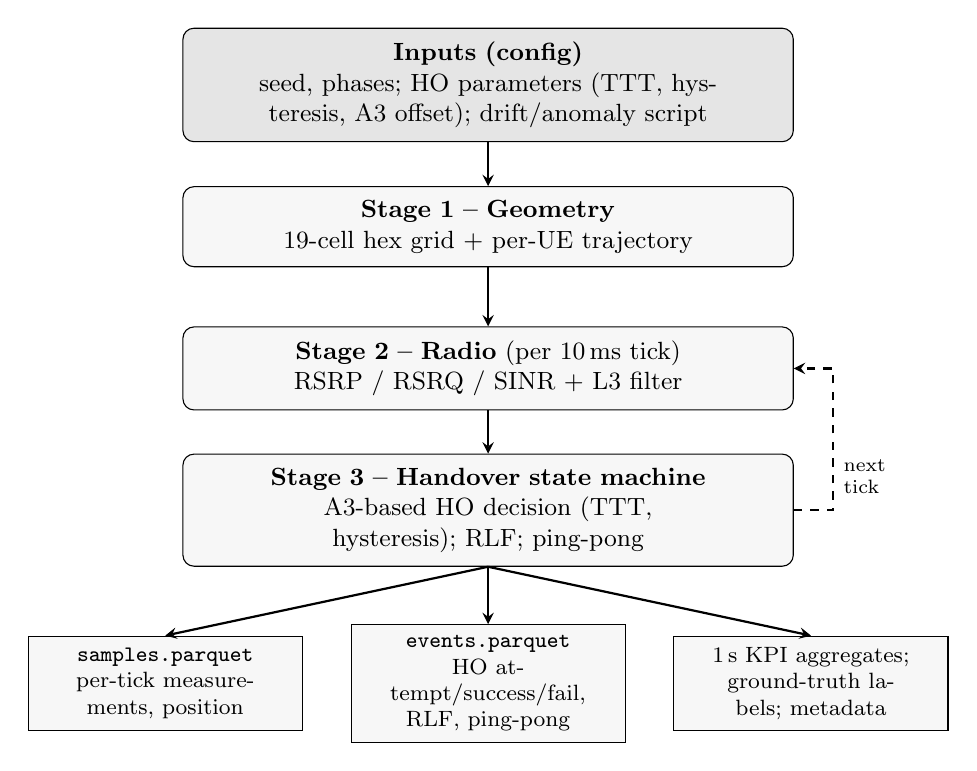
\begin{tikzpicture}[
  font=\small,
  box/.style={rectangle, rounded corners, draw, align=center, text width=7.4cm,
              inner sep=5pt, minimum height=9mm, fill=black!3},
  io/.style={rectangle, rounded corners, draw, align=center, text width=7.4cm,
             inner sep=5pt, minimum height=9mm, fill=black!10},
  ofile/.style={rectangle, draw, align=center, text width=3.2cm, font=\footnotesize,
                inner sep=4pt, minimum height=12mm, fill=black!3},
  arr/.style={->, >=stealth, thick}
]
% configuration input and the three-stage pipeline (central column)
\node[io]  (in) at (0,0)    {\textbf{Inputs (config)}\\ seed, phases; HO parameters (TTT, hysteresis, A3 offset); drift/anomaly script};
\node[box] (s1) at (0,-1.8) {\textbf{Stage 1 -- Geometry}\\ 19-cell hex grid $+$ per-UE trajectory};
\node[box] (s2) at (0,-3.6) {\textbf{Stage 2 -- Radio} (per 10\,ms tick)\\ RSRP / RSRQ / SINR $+$ L3 filter};
\node[box] (s3) at (0,-5.4) {\textbf{Stage 3 -- Handover state machine}\\ A3-based HO decision (TTT, hysteresis); RLF; ping-pong};
% outputs, split into the separate artefacts the run writes
\node[ofile] (o1) at (-4.1,-7.6) {\texttt{samples.parquet}\\ per-tick measurements, position};
\node[ofile] (o2) at ( 0.0,-7.6) {\texttt{events.parquet}\\ HO attempt/success/fail, RLF, ping-pong};
\node[ofile] (o3) at ( 4.1,-7.6) {1\,s KPI aggregates;\\ ground-truth labels; metadata};
\draw[arr] (in) -- (s1);
\draw[arr] (s1) -- (s2);
\draw[arr] (s2) -- (s3);
\draw[arr] (s3.south) -- (o1.north);
\draw[arr] (s3.south) -- (o2.north);
\draw[arr] (s3.south) -- (o3.north);
\draw[arr, dashed] (s3.east) -- ++(0.5,0) |- (s2.east)
      node[pos=0.12, right, font=\scriptsize, align=left]{next\\ tick};
\end{tikzpicture}
\caption[Data flow of the 5G NR SA handover simulator]{Data flow of the 5G NR SA
handover simulator. Configuration and a scenario script (drift and anomaly
injection) drive three stages: \emph{geometry} (19-cell hexagonal grid, each
cell a separate gNB, with a per-UE Random-Direction trajectory); per-tick
\emph{radio} modelling (RSRP/RSRQ/SINR from the TR~38.901 channel model with
LoS/NLoS, path loss and spatially correlated shadowing, smoothed by the layer-3
filter); and the \emph{handover state machine} (Event~A3 with time-to-trigger,
the T310/N310/N311 radio-link-failure timers, and ping-pong detection). The loop
is evaluated per 10\,ms tick and writes three parquet artefacts together with
ground-truth labels and metadata for the analysis pipeline (own elaboration).}
\label{fig:simulator-flow}
\end{figure}

\paragraph{Topology and deployment.}
The scenario is a 19-cell two-tier hexagonal grid (a centre cell plus two
surrounding rings of six and twelve), with an inter-site distance of 500\,m and
an omnidirectional antenna at each cell centre. The layout and inter-site distance follow the 3GPP Urban
Macro reference scenario~\cite{tr38913}; the radio settings use common
urban-macro evaluation assumptions: carrier 3.5\,GHz (band n78), 100\,MHz
bandwidth carried on 273 resource blocks at 30\,kHz subcarrier
spacing~\cite{ts38104}, base-station height 25\,m and UE height 1.5\,m (the
TR~38.901 UMa defaults~\cite{tr38901}), transmit power 49\,dBm, antenna gain
8\,dBi and a UE noise figure of 7\,dB. Each
of the 19 cells is treated as a separate gNB, so every handover the simulator
produces is, by construction, an inter-gNB Xn handover.

\paragraph{Trajectory.}
Each UE moves in a straight line at a constant speed: it starts at a random point
inside the deployment area, picks a random direction, and walks for the duration
of the phase, so its displacement is exactly speed times duration. This keeps the
ground truth simple and reproducible (everything is fixed by the seed). When a
long timeline carries a UE from one phase into the next, only its end position is
kept and a fresh direction is drawn for the new phase (the Random-Direction
model). Re-drawing the direction matters in practice: keeping the same heading
made UEs walk in a straight line off the cell footprint after a few phases and
collapse the received power, so the direction is reset at every phase boundary,
and any UE that would leave the area is simply respawned at a random point.

\paragraph{Radio measurements.}
For every tick and every cell, the simulator computes RSRP, RSRQ and SINR from
the 3GPP TR~38.901 channel model~\cite{tr38901}.
First, a line-of-sight (LoS) or non-line-of-sight (NLoS) state is drawn per cell
from the TR~38.901 LoS-probability formula and is correlated over distance so it
does not flicker tick to tick. Second, the path loss is the TR~38.901 Urban Macro
formula (Table~7.4.1-1), which is a two-slope function of distance with a
breakpoint and a separate, higher NLoS branch. Third, shadow fading is added as a
spatially correlated random field: rather than drawing an independent value per
sample, the simulator builds a smooth two-dimensional field (decorrelation
distance 37\,m, standard deviation 4\,dB in LoS and 6\,dB in NLoS) so that nearby
positions see similar fading, as real shadowing does. From these, RSRP is the
transmit EIRP minus path loss minus shadowing (normalised to a single resource
element), the wideband RSSI is the sum of all cell powers plus thermal noise, and
RSRQ and SINR follow their standard definitions (RSRQ $= N\cdot$RSRP$/$RSSI; SINR
$=$ serving-cell power over the sum of the other cells plus noise), consistent
with TS~38.215~\cite{ts38215}. The Urban Micro street-canyon model is implemented
as the alternative used by the channel-swap drift scenario (D-2). Fast
(symbol-level) fading is not modelled, because it averages out over the
measurement window and does not affect handover-event timing.

\paragraph{Handover state machine.}
The control plane is evaluated once per 10\,ms tick and follows the NR procedure
clause by clause. The raw per-cell measurements are first smoothed by the
layer-3 filter of TS~38.331~\S5.5.3.2, an exponential moving average
$F_n = (1-\alpha)F_{n-1} + \alpha M_n$ with the standard
$\alpha = 1/2^{k/4}$ ($k=4$, i.e.\ $\alpha = 0.5$). On the filtered values the
simulator evaluates Event~A3 of TS~38.331~\S5.5.4.4, whose entry condition is
that a neighbour exceeds the serving cell by the hysteresis plus the A3 offset
($M_n - \mathrm{Hys} > M_s + \mathrm{Off}$; the per-cell offset terms are set to
zero in this work). A neighbour that satisfies the condition accumulates time;
once it has held for the time-to-trigger, a handover to that neighbour fires (at
most one per tick), the UE spends a short execution interval detached, and on
completion the target becomes the serving cell. In parallel, radio-link failure
is tracked by the T310 state machine of TS~38.331~\S5.3.10: when the serving SINR
stays below an out-of-sync threshold ($-8$\,dB) for $N310=6$ ticks the T310 timer
(1\,s) starts, recovery needs $N311=2$ in-sync ticks above $-6$\,dB, and if T310
expires an RLF is declared and the UE re-establishes on the strongest cell.
Finally, a handover that returns the UE to the cell it just left within a short
window is logged as a ping-pong, in line with the mobility-robustness conventions
of TR~36.839~\cite{ts38331,tr36839}. The baseline configuration is TTT~256\,ms,
hysteresis 2\,dB and A3 offset 0\,dB. One simplification is worth stating: the
10\,ms tick is finer than the spec's $\approx$200\,ms layer-1 measurement period,
so the filter and the failure counters react somewhat faster than in a real UE;
the logic is faithful, the time constants are not.

\paragraph{Outputs.}
Each run writes two parquet streams plus a metadata file. \texttt{samples.parquet}
holds the per-UE, per-tick radio measurements and position;
\texttt{events.parquet} is the per-event log of handover attempt, success and
failure, RLF and ping-pong, each row carrying the active control parameters and
pre/post signal snapshots. A one-second per-cell aggregate (RSRP/SINR
percentiles, event counts, HOSR) is also produced for the drift streams. A single
schema with canonical \texttt{snake\_case} names is shared by the simulator and
the Python pipeline, so the same column means the same thing everywhere.

\section{Calibration against real measurements}
\label{sec:calibration}

Calibration is intended to show that the simulator's radio layer produces
distributions broadly \emph{compatible} with real 5G measurements; this is
sufficient when the simulator is used as independent training data, and no
stronger claim of statistical identity is made. The serving-cell RSRP, RSRQ
and SINR marginals are compared against the NordicDat \texttt{op1/5G-NSA/LTE\_B20}
segment with the two-sample Kolmogorov--Smirnov statistic
(\texttt{scipy.stats.ks\_2samp}), the two-sample form of the classical KS
goodness-of-fit statistic~\cite{massey1951ks}. The KS statistic, together
with a 200-replicate bootstrap 95\% confidence interval and the median offset
$\Delta p_{50}$ (sim median minus real median), is the reported quantity.
P-values are deliberately not used as the headline metric: at tens of thousands
of samples per side any non-zero KS statistic gives a vanishing p-value, so it
carries no information at this scale.

A $3\times3$ grid over inter-site distance and trajectory area indicated that the
default TR~38.901 configuration, chosen before inspecting the real data, already
provides the closest fit among the grid points. RSRP and SINR match closely
(KS~0.175 and 0.192, median offsets $+3.1$\,dB and $-2.2$\,dB). RSRQ retains a
residual mismatch (KS~0.467)
that is insensitive to channel parameters; it is load-driven rather than
channel-driven, since the v0 model uses a deterministic interference assumption,
and it is documented as a known limitation. The handover control plane itself is
\emph{not} calibrated against real handover logs, because no public 5G~SA
handover-event dataset exists; instead it is verified against the specification
through the simulator's unit tests.

\section{Scenario design: drift and anomaly injection}
\label{sec:scenarios}

A key advantage of the simulator is that drift and anomalies can be introduced at
controlled times with ground-truth labels, which is difficult to obtain from real
data. A \emph{timeline} is a concatenation of phases: a clean baseline warm-up so the
detectors can learn ``normal'', a sequence of drift and anomaly phases separated
by baseline-recovery gaps, and a steady-state tail for post-drift evaluation.

\paragraph{Drift scenarios.}
Four intra-NR drift types are scripted, each starting from baseline and applying
one transformation at a phase boundary: D-1 traffic-load shift (UE-density
change), D-2 channel-model swap (UMa~$\rightarrow$~UMi, i.e.\ cell
densification), D-3 mobility shift (mean UE speed change, e.g.\ $10\rightarrow25$\,m/s),
and D-4 reconfiguration (the operator pushes new TTT/hysteresis/A3-offset
values). D-4 changes only the control plane and therefore provides the most
direct signal for the configuration--performance surrogate. All four are
intra-5G-NR and stay within the scope defined in Section~\ref{sec:design}.

\paragraph{Anomaly scenarios.}
Four anomaly types are injected. These are the ground-truth events that the five
detectors of Section~\ref{sec:anomaly-method} are later asked to recover (the
count of four refers to the injected fault types, not to the number of
detectors). Each type corrupts the per-UE measurement stream before the handover
loop runs, so that the injection produces genuine downstream effects rather than
only a flag in a table. A-1 (RLF burst) lowers the SINR on all cells for the
affected UEs by enough to push the serving cell below the failure threshold; A-2
(measurement glitch) freezes the UE's RSRP at a constant value, mimicking a stuck
sensor; A-3 (interference spike) subtracts SINR from specific cells, so every UE
that sees those cells is affected; and A-5 (slow degradation) adds a slow linear
SINR decline on a single UE. Each injection is labelled with its time window and
the UEs and/or cells it affects, and this label is the ground truth for the
detection benchmark.

\paragraph{Timelines and labelling.}
Production timelines are generated deterministically by a parametric generator
(\texttt{tools/gen\_timeline.py}) given a seed and the desired number of phases,
drifts and anomalies; anomalies are forbidden in the head-baseline phases so the
detectors always get a clean training window. The main timeline used for the
benchmarks, \texttt{timeline\_medium}, has 30 phases of 60\,s (1\,800\,s total),
eight drifts (two per type) and forty anomalies (ten per type), with UE
carry-over enabled. Building a timeline emits the two parquet streams plus
\texttt{ground\_truth\_\allowbreak drift.parquet} and
\texttt{ground\_truth\_\allowbreak anomaly.parquet},
whose time bounds are rewritten to timeline-global seconds so detectors can join
against them cleanly. Each timeline is fully reproducible from its config JSON,
master seed and simulator git SHA.

\section{Static configuration sweep}
\label{sec:sweep}

To learn the configuration--performance relationship independently of any
timeline, a separate static sweep varies the handover parameters on an otherwise
fixed environment. The grid is TTT~$\in\{256,480,1024\}$\,ms, hysteresis
$\in\{0,2,4,6\}$\,dB and A3 offset $\in\{0,3,6\}$\,dB, each of the 36 unique
configurations repeated over 10 random seeds, giving 360 runs executed in
parallel (\texttt{parfor}). Each run records the controlled parameters, the seed,
the resulting radio context and the mobility KPIs, and the result is written as
the training matrix for the surrogate model (Section~\ref{sec:surrogate}).

\section{Anomaly detection}
\label{sec:anomaly-method}

This layer is deliberately formulated as an \emph{unsupervised anomaly-detection}
problem on windowed multivariate KPI time series, and not as a supervised
data-stream \emph{classification} task. No anomaly labels are used during
training: each detector learns a model of normal handover behaviour and scores
how far a window deviates from it~\cite{chandola2009anomaly}, and the
injected-anomaly labels are used only for evaluation. This choice reflects the
operational setting, where labelled handover faults are not available ahead of
time and ``abnormal'' must be defined relative to recent normal behaviour rather
than to a fixed set of fault classes.

\paragraph{Window features.}
Detection operates on fixed-length sliding windows rather than raw samples.
Samples are aggregated into 5\,s windows with a 1\,s slide, and windows never
cross a (UE, phase) boundary. For each of the six radio/mobility numeric columns
(serving and neighbour RSRP/RSRQ, serving SINR, and UE speed) the window
records the 10th, 50th and 90th percentiles and the standard deviation; the
modal serving cell, the five event-type counts (HO attempt/success/fail, RLF,
ping-pong) and four derived rates (HOSR, HO-failure, RLF and ping-pong rate) are
added, for a 34-dimensional feature vector. These features are grouped into
seven disjoint families (RSRP, RSRQ, SINR, speed, cell, events, derived) used by
the ablation study. Only mobility-layer columns are consumed, consistent with the
KPI scope of Section~\ref{sec:design}.

\paragraph{Detectors.}
Five unsupervised detectors are compared, one per major detection family, each
behind a shared median-imputation and standardisation pipeline fitted on the
training data only: Isolation Forest (200 trees), Local Outlier Factor (20
neighbours, novelty mode), One-Class SVM (RBF kernel, $\nu=0.05$),
PCA-reconstruction error (truncated SVD, 5 components) and an MLP autoencoder
(bottleneck $16$-$8$-$16$, early stopping)~\cite{liu2008isolation,breunig2000lof,scholkopf2001ocsvm,jolliffe2002pca,shyu2003pca}.
All scores follow the convention that higher means more anomalous. The
implementations are from \texttt{scikit-learn}~\cite{pedregosa2011scikit}.

\paragraph{Training and labelling.}
Training is unsupervised: each detector is fitted only on clean
baseline windows (the first three phases, with all labelled-anomaly windows
removed), and then scores the entire timeline. A window is labelled positive
when it overlaps an injected anomaly in time \emph{and} matches its UE and cell
scope, which gives both an overall anomaly label and per-type labels.

\paragraph{Evaluation.}
The primary metric is the area under the precision--recall curve (PR-AUC), with
ROC-AUC recorded in the accompanying result artefacts; precision--recall is
preferred because anomalies are rare. The task is in fact strongly imbalanced: at the 5\,s window the positive
(anomalous) windows account for only about $2.4$--$7.0\%$ of the windows of a
given anomaly type (roughly $159$--$376$ positive against $5\,000$--$7\,200$
negative windows, i.e.\ an imbalance ratio between about $1{:}13$ and $1{:}41$).
The random-classifier PR-AUC baseline therefore equals the positive prevalence
itself ($\approx 0.02$--$0.07$), and the reported PR-AUC values should be read
against this low baseline rather than against~$1$; accuracy and raw precision
are not used precisely because they are dominated by the majority (normal)
class. Confidence intervals are obtained by stratified bootstrap (1\,000
resamples, 95\% interval), resampling positives and negatives separately.
PR-AUC is reported per anomaly type and pooled over the timeline. Two robustness
analyses accompany the headline numbers: a window-size sweep over
$\{2,5,10,30\}$\,s, and a drop-one-family ablation on the best detector that
reports the change in PR-AUC when each feature family is removed. A per-phase
false-positive / true-positive figure with drift phases shaded shows how a
static detector degrades as the environment drifts, which motivates the adaptive
layer.

\section{Drift detection}
\label{sec:drift-method}

\paragraph{Streams.}
Drift detection runs on six fleet-level univariate time series sampled at 1\,Hz:
the per-second fleet means of serving RSRP and serving SINR, and four rolling
(10\,s window) event rates, namely HO attempt rate, HOSR, ping-pong rate and RLF
rate. A UE-speed stream is deliberately excluded, since it would make the
mobility drift trivially detectable.

\paragraph{Detectors.}
Seven detectors, spanning the three families of
Section~\ref{subsec:drift-methods}, are benchmarked: ADWIN, Page--Hinkley and
KSWIN (sequential statistics on the raw stream), DDM and EDDM (error-rate
detectors over a binarised stream), and MMD-batch and Energy-batch (sliding
two-sample tests). The streaming and binarised detectors use the
\texttt{river} library~\cite{montiel2021river}; the batch tests use an RBF-kernel
MMD and the energy distance with a permutation test, comparing a locked
reference window to a sliding active window. Each detector exposes a uniform
\texttt{update(value)$\rightarrow$bool} interface and skips missing values, and a
fresh instance is used per stream (seven detectors $\times$ six streams).

\paragraph{Evaluation.}
A stream second is labelled as drift when it lies in an injected drift interval
\emph{and} the stream's KPI is among those the drift is expected to affect. For
each drift instance and each detector/stream pair, detection latency is the time
from the drift onset to the first firing inside an eligibility window that
extends 30\,s past the drift, and a missed detection is recorded if no firing
occurs in that window. Three quantities are reported: detection latency
(bootstrap median over 1\,000 resamples with a 95\% interval, taking each
detector's best stream), miss rate, and a baseline false-positive rate measured
as false alarms per second on the clean baseline phases. Together these capture
the latency--false-alarm trade-off across detectors.

\section{Drift-aware adaptive monitoring}
\label{sec:adaptive-method}

The adaptive layer tests whether refreshing the anomaly monitor when drift is
detected recovers the accuracy that a static monitor loses after drift. The base
detector is the PCA-reconstruction monitor and the trigger is an ADWIN detector
($\delta=0.01$) watching the HOSR and RLF-rate streams. After a warm-up fit on
the clean baseline phases, four retraining strategies that share this base and
trigger are compared:

\begin{itemize}
  \item \textbf{Static}: never refit after warm-up (the baseline).
  \item \textbf{Periodic}: refit every 180\,s regardless of drift.
  \item \textbf{Drift-triggered naive}: refit when ADWIN fires (subject to a
  30\,s cooldown), using the recent window as-is.
  \item \textbf{Drift-triggered filtered}: same trigger, but the retraining pool
  is first cleaned with a self-supervised filter that scores the pool with the
  current detector and keeps only the bottom 80\% (lowest-scoring, ``currently
  normal'') windows, dropping the top 20\% the model already considers
  suspicious.
\end{itemize}

For all non-static strategies the retraining pool is the last 120\,s of windows
ending at the trigger time, taken \emph{without} labels to reflect operational
reality. The whole layer is evaluated in a \emph{prequential}
(test-then-train) fashion: each window is first scored by the current monitor
and only afterwards may it enter a retraining pool, so the monitor is always
tested on data it has not yet been fitted on. Performance is tracked as a sliding
PR-AUC (120\,s window, 30\,s stride), reported both pooled over the whole
post-warm-up timeline and restricted to the drift phases, alongside a cost ledger
(number of refits, training samples and CPU time). The filtered strategy is accepted if its overall
PR-AUC is at least that of periodic retraining and its drift-phase PR-AUC
exceeds the static monitor's by at least 0.10. This comparison is designed to
show whether naive retraining degrades the monitor by absorbing post-drift
anomalies into ``normal'', and whether the self-supervised filter mitigates this.

\section{Configuration--performance surrogate}
\label{sec:surrogate}

The surrogate learns the mapping from handover configuration to mobility outcome,
which is what makes a reconfiguration recommendation possible. It is trained on
the 360-row static sweep (Section~\ref{sec:sweep}). The inputs are the three
controlled parameters (TTT, hysteresis, A3 offset) plus nine
deployment-context features (RSRP/SINR/RSRQ at the 10th/50th/90th percentiles),
and the three targets are HOSR, RLF rate and ping-pong rate (handover-failure
rate is omitted as the complement of HOSR).

The surrogate has two heads. A histogram gradient-boosting regressor
(\texttt{HistGradient\-Boosting\-Regressor}, 500 iterations, learning rate 0.05,
depth 6) provides the point estimate~\cite{pedregosa2011scikit}. For
uncertainty, a quantile gradient-boosting model is wrapped in split-conformal
calibration (conformalised quantile regression)~\cite{romano2019cqr}: a
calibration split (35\% of the training portion) is held out, conformity scores
adjust (typically widen) the nominal 5\%/95\% quantile band, and the result is a 90\% prediction
interval with a finite-sample coverage guarantee. Models are evaluated with
grouped 5-fold cross-validation, where all ten seed replicates of a
configuration stay in the same fold so the model is always tested on unseen
configurations. Point accuracy is reported as MAE, RMSE and $R^2$ per target,
and interval quality as the empirical coverage of the 90\% interval, comparing
the naive and the conformal variant against their nominal coverage under grouped
cross-validation.

The surrogate also answers an inverse question. Given a fixed deployment context,
all 36 candidate configurations are scored, those satisfying the operating
constraints (HOSR~$\geq0.95$, RLF rate~$\leq0.05$, ping-pong rate~$\leq0.10$)
are kept, and the feasible set is ranked by predicted HOSR, with the conformal
interval attached for reporting. This inverse query is what recommends a
recovery configuration after a harmful reconfiguration.

\section{End-to-end adaptive loop}
\label{sec:end2end}

The four layers are combined into one replay over \texttt{timeline\_medium} that
exercises the full ``detect~$\rightarrow$~adapt~$\rightarrow$~recommend'' loop and
estimates the performance impact of drift. The PCA-AE monitor with the
ADWIN trigger runs the drift-triggered-filtered strategy; whenever a drift is
detected, the deployment context is summarised from the last 60\,s of samples,
the current configuration is read from the most recent event, and the surrogate
inverse query proposes a configuration that maximises predicted HOSR under the
operating constraints. The benefit of each intervention is reported as a
\emph{counterfactual KPI uplift}: the difference between the surrogate's
predictions for the recommended and the current configuration in the same
context, signed so that a positive value is always an improvement, with the
conformal 90\% interval on the recommended configuration. Rather than only
testing whether drift changes HOSR at the segment level, this loop estimates how
much a fixed configuration may underperform after drift and whether a feasible
reconfiguration would be expected to recover it.

\section{External validation}
\label{sec:external}

Three independent checks probe how far the results generalise. A cross-seed
replication reruns the whole pipeline on five master seeds and aggregates each
headline metric with a bootstrap confidence interval. A cross-scenario check
repeats the benchmarks on a denser urban timeline and compares the deltas. A
real-data face-validity check runs the PCA-AE monitor and ADWIN, fully
self-supervised and with no simulator-trained weights transferred, on the
NordicDat 5G-NSA operator segment; because that data has no ground truth, only
volume-sanity and temporal-plausibility are claimed (for example, the fraction
of flagged windows and whether flagging peaks at plausible commute hours), and
no precision or recall is reported.

\section{Implementation, tools and reproducibility}
\label{sec:tools}

The simulator is written in MATLAB R2023b (Communications, 5G, Statistics and
Machine Learning, and Parallel Computing toolboxes). The analysis pipeline is
Python~3.12 and uses \texttt{scikit-learn} for the anomaly detectors, PCA and
gradient boosting, \texttt{river} for the streaming drift
detectors~\cite{montiel2021river}, \texttt{scipy} for the KS and energy-distance
statistics, \texttt{pandas}/\texttt{pyarrow} for parquet I/O and
\texttt{matplotlib} for figures. The pipeline is designed to be reproducible:
each phase has a single \texttt{make} target, Python dependencies are pinned in a
hash-locked lockfile, simulator artifacts and an SHA256 manifest are archived as
a citable deposit, and the analysis figures can be regenerated from the cached
simulator output without a MATLAB licence. Each timeline and sweep records its
seed and git SHA, so runs are reproducible.


% !TEX encoding = UTF-8 Unicode
% !TEX root = thesis.tex

\chapter{Results and Discussion}
\label{ch:results}

This chapter reports the results of the four analysis layers and the external
validation, and discusses what they mean. Unless stated otherwise, all numbers
are computed on the \texttt{timeline\_medium} timeline (30 phases, 1\,800\,s,
eight drifts, forty anomalies) with the protocols of
Chapter~\ref{ch:method}. Each section maps to one research question:
anomaly detection (RQ1), drift detection (RQ2), drift-aware maintenance (RQ3),
and the configuration--performance link with reconfiguration (RQ4); a final
section reports how well the findings generalise.

\section{Anomaly detection (RQ1)}
\label{sec:res-anomaly}

Table~\ref{tab:anomaly-type} reports the per-type precision--recall AUC (PR-AUC)
of the five detectors, and Table~\ref{tab:anomaly-overall} the pooled PR-AUC over
the whole timeline with 95\% bootstrap intervals. The pattern is fairly
consistent: the two anomalies that leave a clear, structured signature are
detected reasonably well, while the two subtle ones sit close to the noise floor.

\begin{table}[ht]
\centering
\caption{Per-type anomaly PR-AUC at the 5\,s window (best per row in bold; own elaboration).}
\label{tab:anomaly-type}
\begin{tabular}{@{}lrrrrr@{}}
\toprule
Anomaly type & IsoForest & LOF & OCSVM & PCA-AE & MLP-AE \\
\midrule
Measurement glitch  & 0.635 & 0.842 & \textbf{0.858} & 0.784 & 0.756 \\
RLF burst           & 0.616 & 0.703 & 0.685 & \textbf{0.751} & 0.655 \\
Interference spike  & 0.069 & \textbf{0.152} & 0.099 & 0.111 & 0.078 \\
Slow degradation    & 0.045 & 0.038 & 0.045 & \textbf{0.048} & 0.036 \\
\bottomrule
\end{tabular}
\end{table}

\begin{table}[ht]
\centering
\caption{Pooled anomaly PR-AUC over the whole timeline, with 95\% bootstrap CI (own elaboration).}
\label{tab:anomaly-overall}
\begin{tabular}{@{}lr@{}}
\toprule
Detector & Pooled PR-AUC [95\% CI] \\
\midrule
IsoForest   & 0.425 [0.391, 0.460] \\
PCA-AE      & 0.262 [0.237, 0.287] \\
MLP-AE      & 0.236 [0.212, 0.262] \\
LOF         & 0.157 [0.149, 0.167] \\
OneClassSVM & 0.154 [0.145, 0.164] \\
\bottomrule
\end{tabular}
\end{table}

Measurement glitch and RLF burst are recovered with PR-AUC in the $0.6$--$0.86$
range, because both leave a structured fingerprint across several features (a
frozen RSRP, or a correlated SINR/RSRQ collapse with extra RLF events).
Interference spike is much harder (best PR-AUC $0.152$, LOF): it is cell-targeted
and short, so only a fraction of the fleet sees it in any window. Even so, these
values must be read against the imbalance of the task
(Section~\ref{sec:anomaly-method}): with a positive prevalence of only about
$2.4\%$ for interference spike, the random-classifier PR-AUC baseline is
$\approx 0.024$, so LOF's $0.152$ is roughly six times the chance level, not a
non-detection. Slow degradation is the only type that stays essentially at
that floor (PR-AUC $\approx 0.04$ against a $\approx 0.037$ baseline) because a
slow ramp on a single UE barely moves a fleet-aggregated window. This separation between
``easy'' and ``subtle'' anomalies is the main observation for RQ1, and is part of
what motivates the adaptive layer of Section~\ref{sec:res-adaptive}.

No single detector performs best everywhere, which is worth noting. By per-type
mean PR-AUC the strongest detector is LOF, whereas by pooled PR-AUC it is
Isolation Forest ($0.425$); the two views differ because the pooled metric is
dominated by the large number of normal windows and by the easy anomalies. A
reasonable reading is that detector choice should follow the anomaly profile of
interest, not a single headline number.

\paragraph{Robustness checks.}
The window-size sweep ($2$--$30$\,s) shifts the per-type numbers but not the
overall picture: the shortest window helps the sharp, localised anomalies
(measurement-glitch PR-AUC rises to $0.919$ for One-Class SVM and interference
spike to $0.195$ for LOF at $2$\,s), while the longest window helps the
anomalies that need time to accumulate evidence (RLF-burst rises to $0.845$ for
PCA-AE at $30$\,s, and slow degradation roughly doubles, though it stays near
the noise floor). The drop-one-family ablation shows that
the RSRQ feature family is the most important by a wide margin: removing it costs
up to $0.33$ PR-AUC on measurement glitch, whereas removing the event-count or
derived-rate families changes little. Figure~\ref{fig:anomaly-degradation} shows
the per-phase false- and true-positive rates with drift phases shaded, making
visible how a static detector drifts off its operating point as the environment
changes.

\begin{figure}[ht]
\centering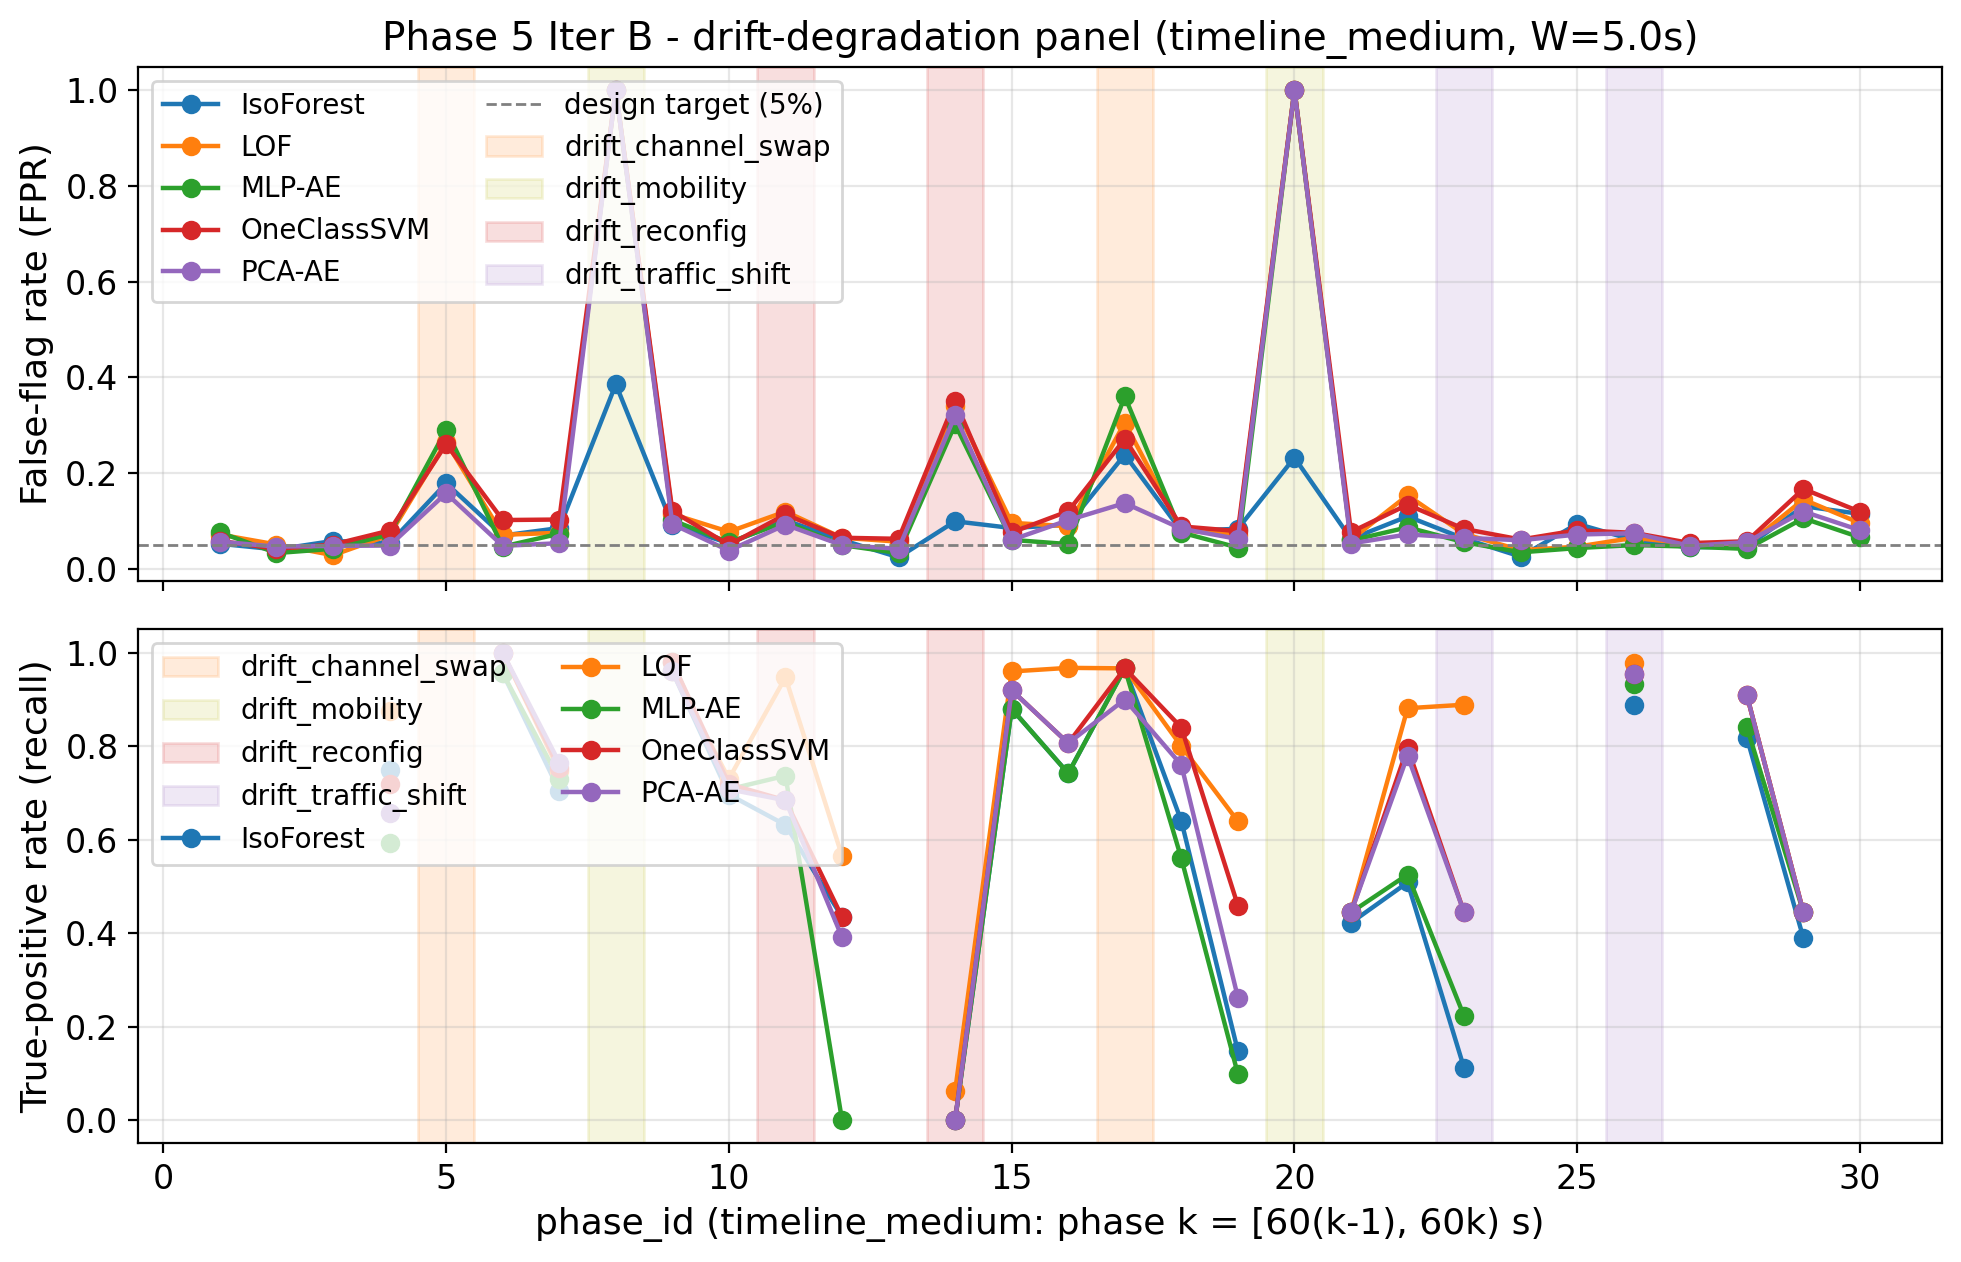
\includegraphics[width=.85\textwidth]{drift_degradation}
\caption{Per-phase false-/true-positive rate of the static anomaly monitor, drift phases shaded (own elaboration).}
\label{fig:anomaly-degradation}
\end{figure}

\section{Drift detection (RQ2)}
\label{sec:res-drift}

Every one of the eight injected drifts is detected by every one of the seven
detectors (instance-level miss rate $0$). What separates the detectors is the
price: how late the alarm comes, and how often it fires on clean data.
Table~\ref{tab:drift} gives the median detection latency per drift type together
with the mean baseline false-alarm rate, and Figure~\ref{fig:drift-heatmap}
visualises the same trade-off.

\begin{table}[ht]
\centering
\caption{Median drift-detection latency (s) per drift type, and mean baseline false-alarm rate (per second) on clean phases (own elaboration).}
\label{tab:drift}
\begin{tabular}{@{}lrrrrr@{}}
\toprule
Detector & Channel & Mobility & Reconfig & Traffic & FPR\,(/s) \\
\midrule
Energy-batch & 3.0  & 3.0  & 3.0  & 3.0  & 0.115 \\
MMD-batch    & 3.0  & 3.0  & 3.0  & 3.0  & 0.117 \\
DDM          & 12.0 & 2.0  & 3.0  & 15.5 & 0.005 \\
Page--Hinkley & 17.0 & 10.5 & 6.0  & 11.5 & 0.011 \\
EDDM         & 25.5 & 3.0  & 7.5  & 5.0  & 0.006 \\
ADWIN        & 23.0 & 19.0 & 13.0 & 29.0 & 0.005 \\
KSWIN        & 51.5 & 20.0 & 20.0 & 24.5 & 0.008 \\
\bottomrule
\end{tabular}
\end{table}

\begin{figure}[ht]
\centering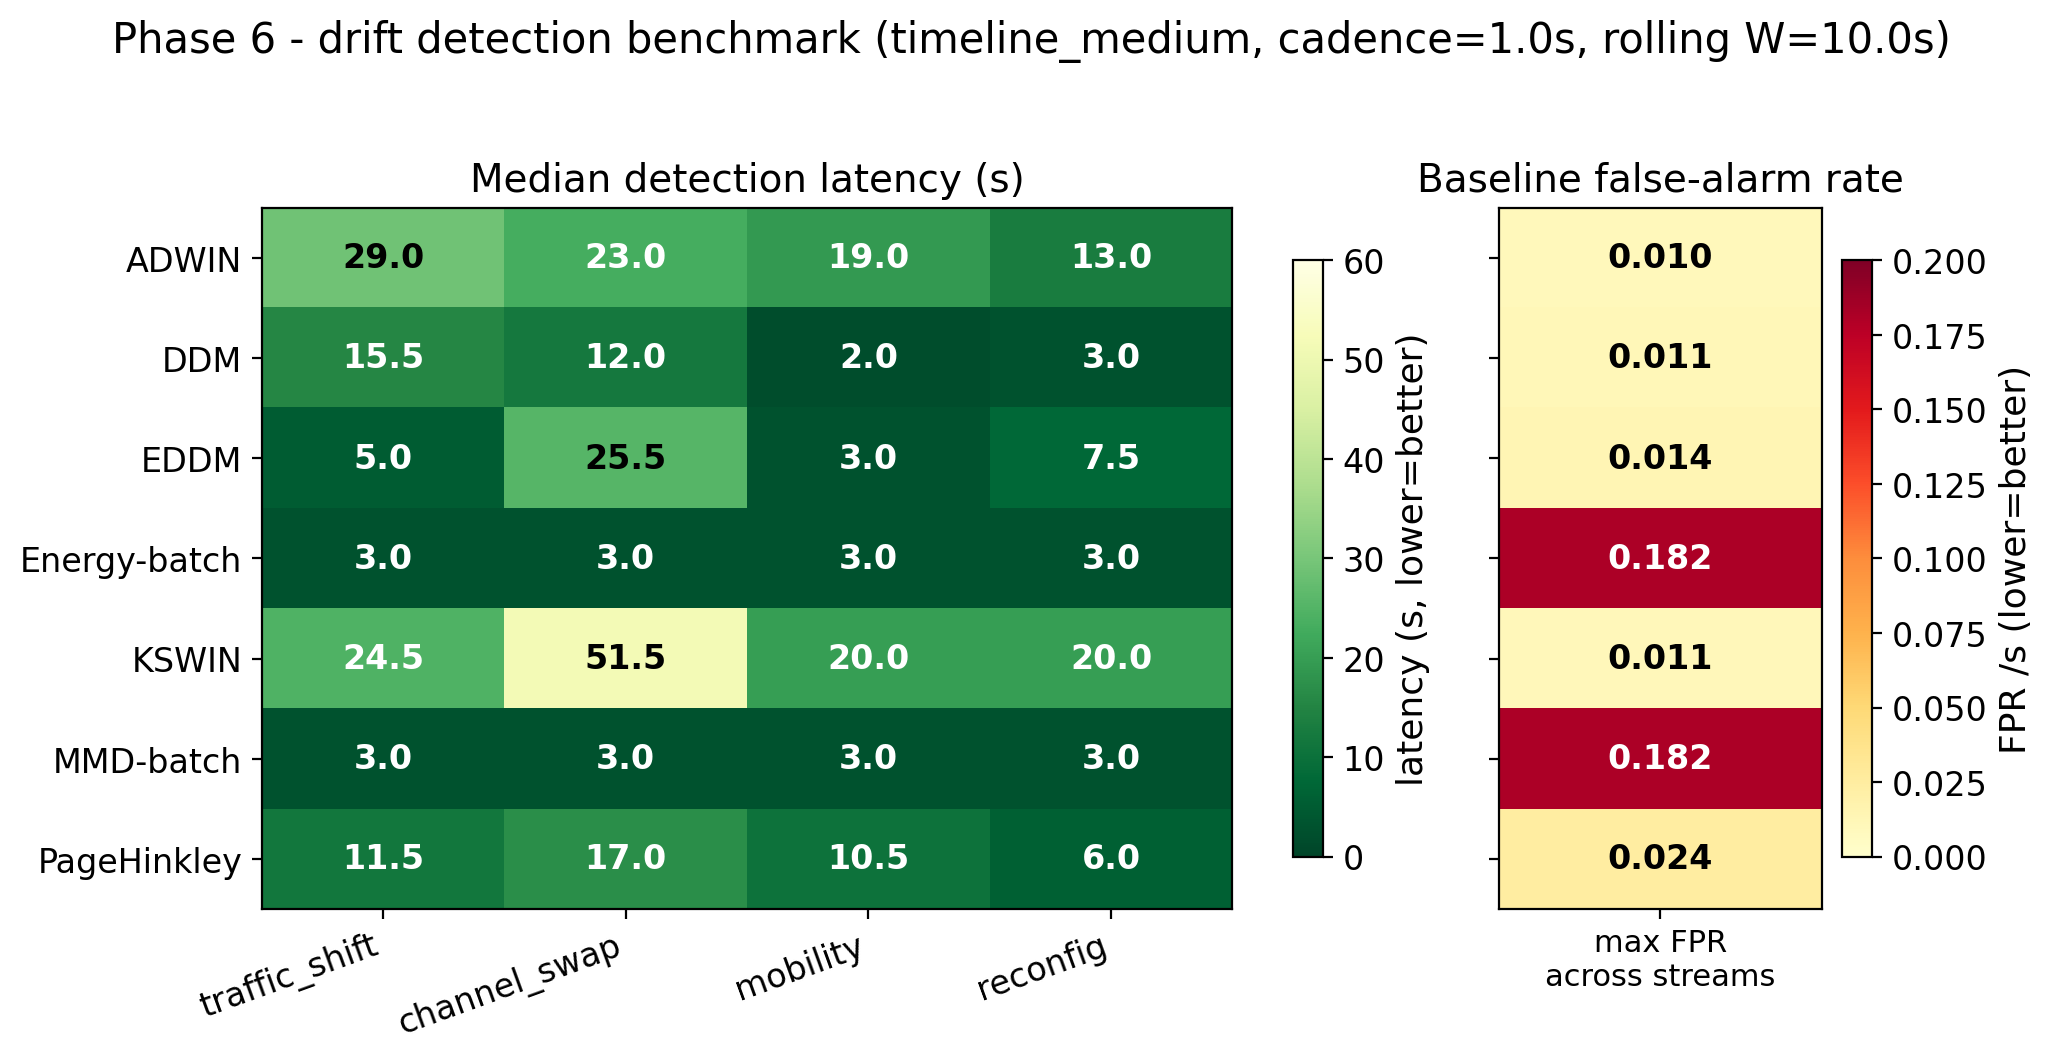
\includegraphics[width=.9\textwidth]{drift_detection_heatmap}
\caption{Drift-detection latency and baseline false-alarm rate per detector and stream (own elaboration).}
\label{fig:drift-heatmap}
\end{figure}

The results point to a latency--false-alarm trade-off. The two batch two-sample
tests, Energy-batch and MMD-batch, react fastest: they flag every drift type in
about $3$\,s, but at the price of a high baseline false-alarm rate
($\approx 0.12$ per second). The sequential and error-rate detectors are the
opposite: ADWIN and DDM keep the baseline false-alarm rate around $0.005$ per
second but take longer, and DDM is notably quick on the abrupt mobility and
reconfiguration drifts ($2$--$3$\,s) where a sharp mean change is present. By the
combined latency criterion (with misses penalised) the overall winner is
Energy-batch, but in an operational setting the low-false-alarm detectors would
be preferable; the right choice depends on whether the cost of a late alarm or a
false alarm is higher. This trade-off, not the crowning of a single best detector, is the
main observation for RQ2.

\section{Drift-aware adaptive monitoring (RQ3)}
\label{sec:res-adaptive}

The PCA-reconstruction detector (PCA-AE) is used as the base monitor for the
adaptive experiments rather than the pooled-best Isolation Forest. The reason is
that the adaptive loop repeatedly refits the detector under drift, so the
selection criterion here is not the highest static accuracy but suitability for
frequent, stable retraining: PCA-AE yields a single continuous
reconstruction-error score that is cheap to refit and behaves consistently across
refits, which makes the quantile-based filtering step (dropping the most
suspicious windows before a refit) well defined. A tree-based score such as
Isolation Forest re-grows its ensemble at every refit and shifts its operating
threshold, which is less suited to the self-supervised filtering used below.

Table~\ref{tab:adaptive} compares the four retraining strategies on the PCA-AE
monitor, and Figure~\ref{fig:adaptive} plots PR-AUC over time. The four
strategies share the same base detector and the same trigger, yet their outcomes
diverge sharply: what appears to decide the result is what is allowed into the
retraining pool.

\begin{table}[ht]
\centering
\caption{Retraining strategies on the PCA-AE monitor (own elaboration).}
\label{tab:adaptive}
\begin{tabular}{@{}lrrrr@{}}
\toprule
Strategy & Overall PR-AUC & Drift-phase PR-AUC & Refits & Train samples \\
\midrule
Static                  & 0.264 & 0.057 & 1 & 2\,016 \\
Periodic                & 0.115 & 0.036 & 9 & 14\,088 \\
Drift-triggered naive   & 0.116 & 0.037 & 8 & 12\,048 \\
Drift-triggered filtered & 0.248 & \textbf{0.187} & 8 & 10\,040 \\
\bottomrule
\end{tabular}
\end{table}

\begin{figure}[ht]
\centering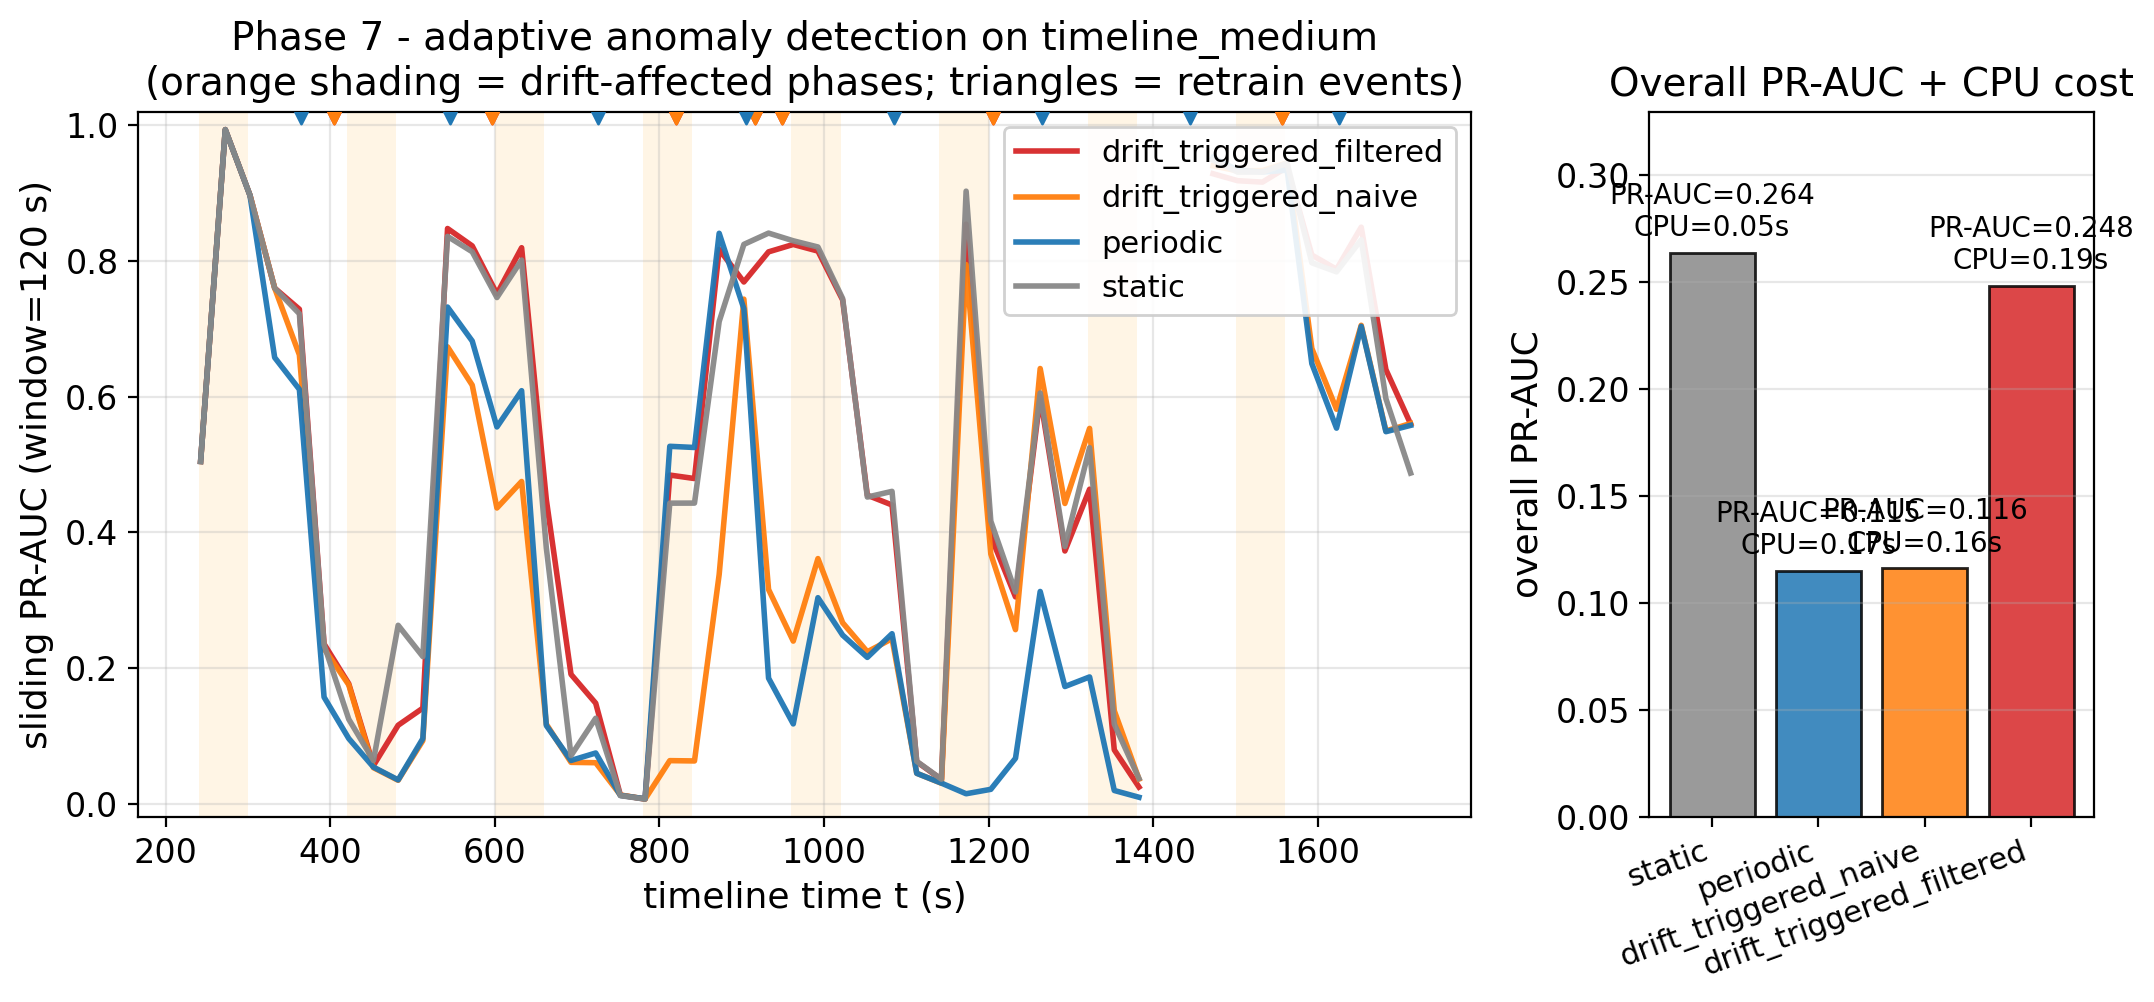
\includegraphics[width=.85\textwidth]{adaptive_pr_auc_over_time}
\caption{Sliding PR-AUC over time for the four strategies, with the cost-versus-gain summary (own elaboration).}
\label{fig:adaptive}
\end{figure}

Naive retraining tends to backfire here. Both periodic and
drift-triggered-naive retraining roughly halve the overall PR-AUC (from $0.264$
to $\approx 0.12$) and barely move the drift-phase PR-AUC. A likely reason is
self-poisoning: because the retraining pool is taken without labels, a refit
triggered just after a drift absorbs the post-drift anomalies into its notion of
``normal'', so the model learns to ignore much of what it should flag. The
self-supervised filter largely addresses this. The drift-triggered-filtered
strategy keeps the overall PR-AUC close to the static baseline ($0.248$ vs
$0.264$) and more than triples the drift-phase PR-AUC ($0.187$ vs $0.057$), a
$+0.13$ improvement that meets the acceptance target of $+0.10$. It also does so
at lower cost than the naive variants (fewer training samples), because the
filter discards the most suspicious windows before refitting. The observation for
RQ3 is therefore a conditional one: in these experiments drift-aware retraining
helps mainly when the retraining data is first cleaned of likely anomalies, while
an unfiltered refit performs worse than not retraining at all.

\section{Configuration--performance and reconfiguration (RQ4)}
\label{sec:res-config}

\paragraph{Surrogate accuracy.}
Table~\ref{tab:surrogate-point} reports the cross-validated accuracy of the
HistGB surrogate on the three mobility KPIs. HOSR and RLF rate are predicted
accurately ($R^2 = 0.96$ and $0.95$; HOSR MAE $0.043$), and ping-pong rate is
harder but still useful ($R^2 = 0.72$). Because the cross-validation is grouped
by configuration, these scores describe performance on configurations the model
has never seen, not memorised training points.

\begin{table}[ht]
\centering
\caption{Surrogate point accuracy, grouped 5-fold CV (own elaboration).}
\label{tab:surrogate-point}
\begin{tabular}{@{}lrrr@{}}
\toprule
Target & MAE & RMSE & $R^2$ \\
\midrule
HOSR           & 0.043 & 0.075 & 0.956 \\
RLF rate       & 0.004 & 0.005 & 0.952 \\
Ping-pong rate & 0.015 & 0.019 & 0.717 \\
\bottomrule
\end{tabular}
\end{table}

\paragraph{Uncertainty calibration.}
Point accuracy is not enough for a recommendation; the intervals must be
trustworthy. Table~\ref{tab:surrogate-cov} shows that the naive quantile
intervals are too narrow under grouped cross-validation: their empirical coverage
of the nominal $90\%$ interval falls to $0.65$--$0.83$. Split-conformal
calibration moves all three targets back towards nominal ($0.72$--$0.89$), at the
cost of slightly wider intervals. Figure~\ref{fig:reliability} shows the same
correction as a reliability diagram. This is why the end-to-end loop reports
conformal rather than naive intervals.

\begin{table}[ht]
\centering
\caption{Empirical coverage of the nominal 90\% prediction interval (own elaboration).}
\label{tab:surrogate-cov}
\begin{tabular}{@{}lrr@{}}
\toprule
Target & Naive coverage & Conformal coverage \\
\midrule
HOSR           & 0.77 & 0.84 \\
RLF rate       & 0.65 & 0.72 \\
Ping-pong rate & 0.83 & 0.89 \\
\bottomrule
\end{tabular}
\end{table}

\begin{figure}[ht]
\centering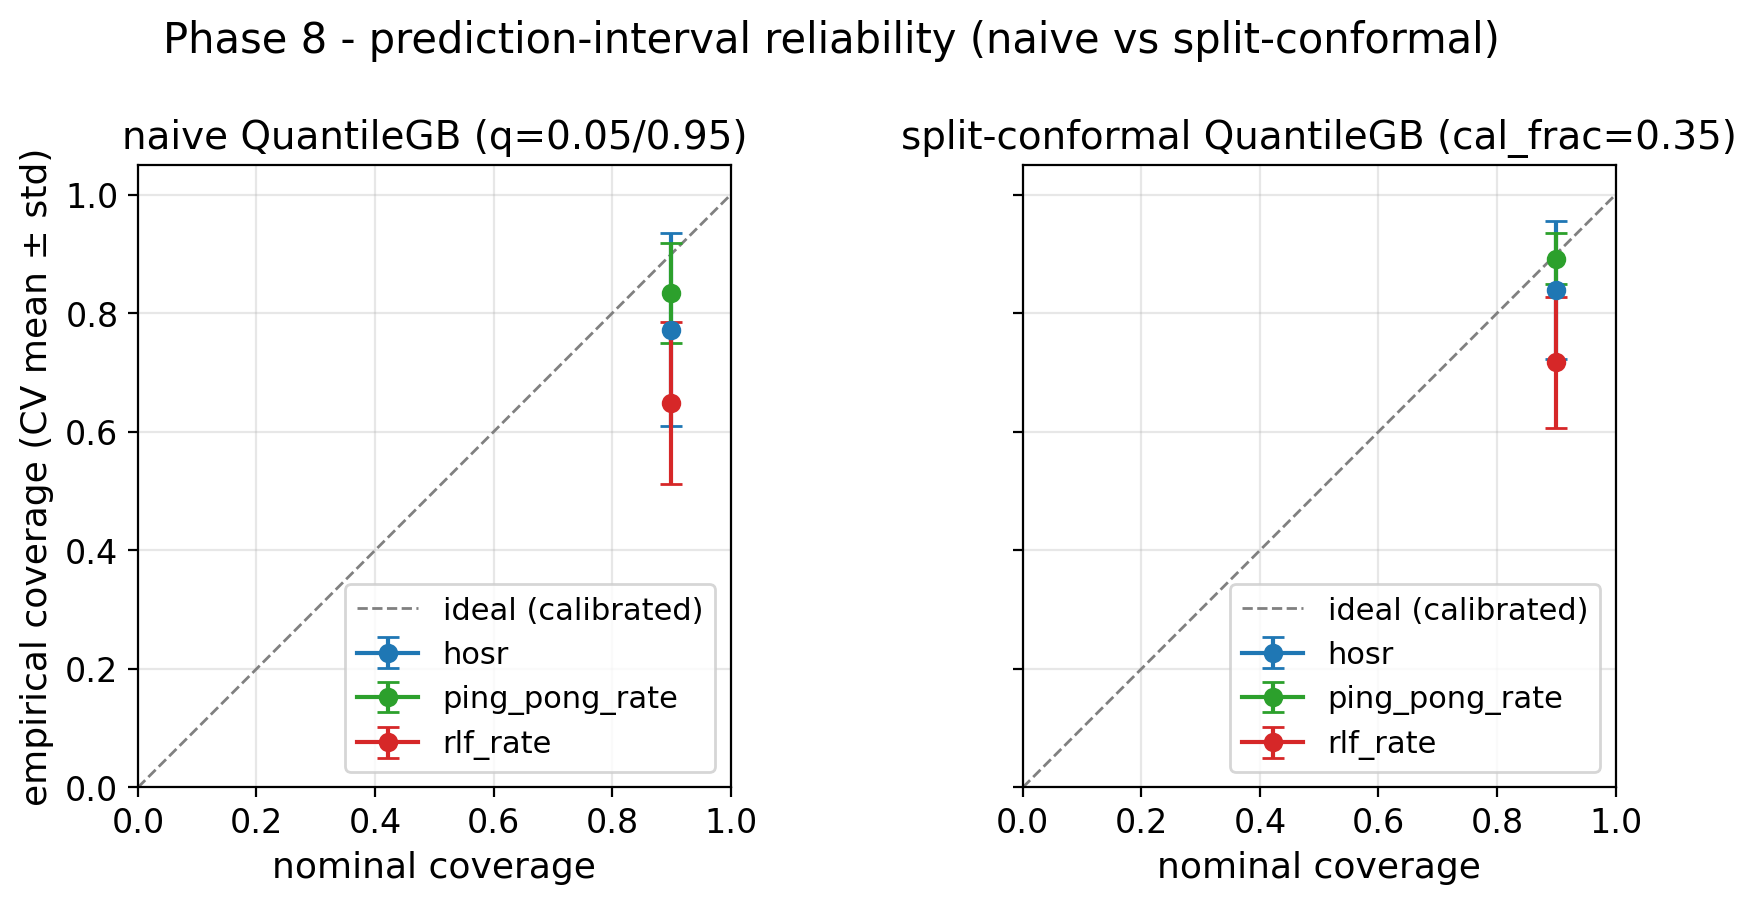
\includegraphics[width=.85\textwidth]{reliability_diagram}
\caption{Naive vs split-conformal interval coverage (own elaboration).}
\label{fig:reliability}
\end{figure}

\paragraph{Inverse query.}
Asked which configuration maximises HOSR under the operating constraints
(HOSR~$\geq0.95$, RLF~$\leq0.05$, ping-pong~$\leq0.10$) at the median deployment
context, the surrogate finds $12$ of the $36$ candidates feasible. The top three
all use the shortest time-to-trigger, TTT~$=256$\,ms (with hysteresis/A3 offset
$(6,0)$, $(2,3)$ and $(0,6)$\,dB), each reaching predicted HOSR~$\approx 1.0$.
The interpretation is that, in this radio context, a fast trigger paired with
enough hysteresis or offset to suppress ping-pong is preferable, and the
surrogate makes that trade-off explicit (Figure~\ref{fig:inverse}).

\begin{figure}[ht]
\centering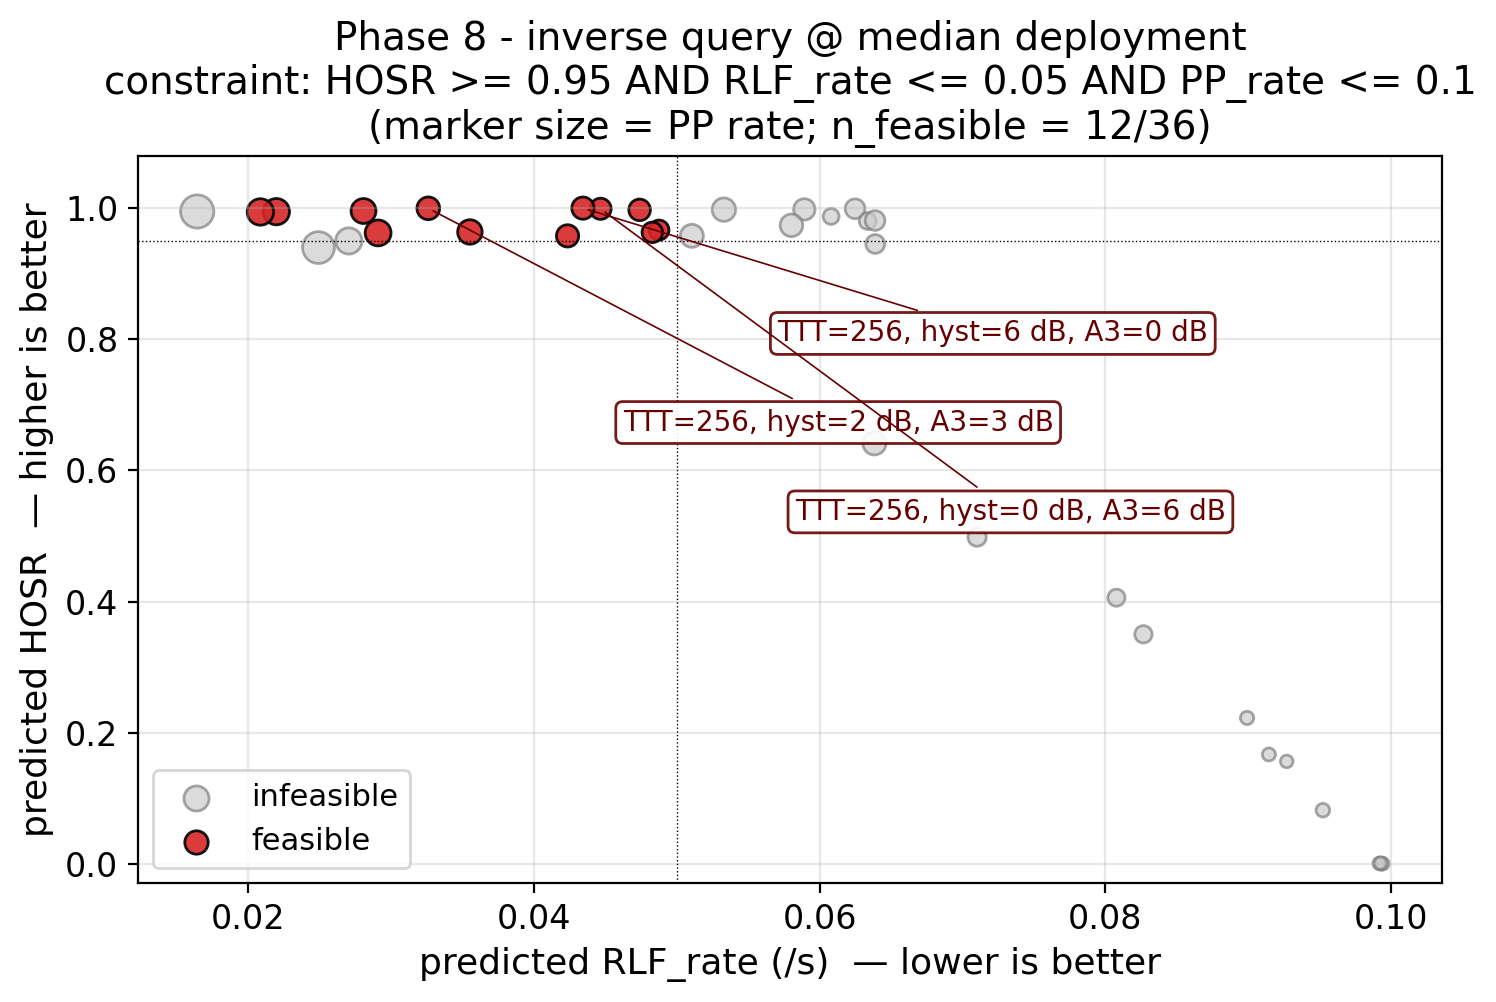
\includegraphics[width=.85\textwidth]{inverse_query}
\caption{Feasible configurations on the HOSR vs RLF plane; top-3 annotated (own elaboration).}
\label{fig:inverse}
\end{figure}

\paragraph{End-to-end reconfiguration.}
Running the full loop over the timeline produces seven drift-triggered
interventions. The most relevant case is the harmful reconfiguration drift
(D-4), where the operator raises the time-to-trigger: the monitor detects it and
the surrogate recommends a recovery configuration, and across all interventions
the cumulative \emph{predicted} HOSR uplift is $+0.62$
(Figure~\ref{fig:end2end}). All four demo acceptance checks pass: at least five
interventions fire, every recommendation lies inside the trained grid, both D-4
events change the configuration, and the cumulative HOSR uplift is positive. This
completes the RQ4 loop: drift can degrade the handover KPI, and a feasible
reconfiguration, chosen from the surrogate, is predicted to recover it. The
uplift is a model prediction, not a measured field gain, which is stated
as a limitation.

\begin{figure}[ht]
\centering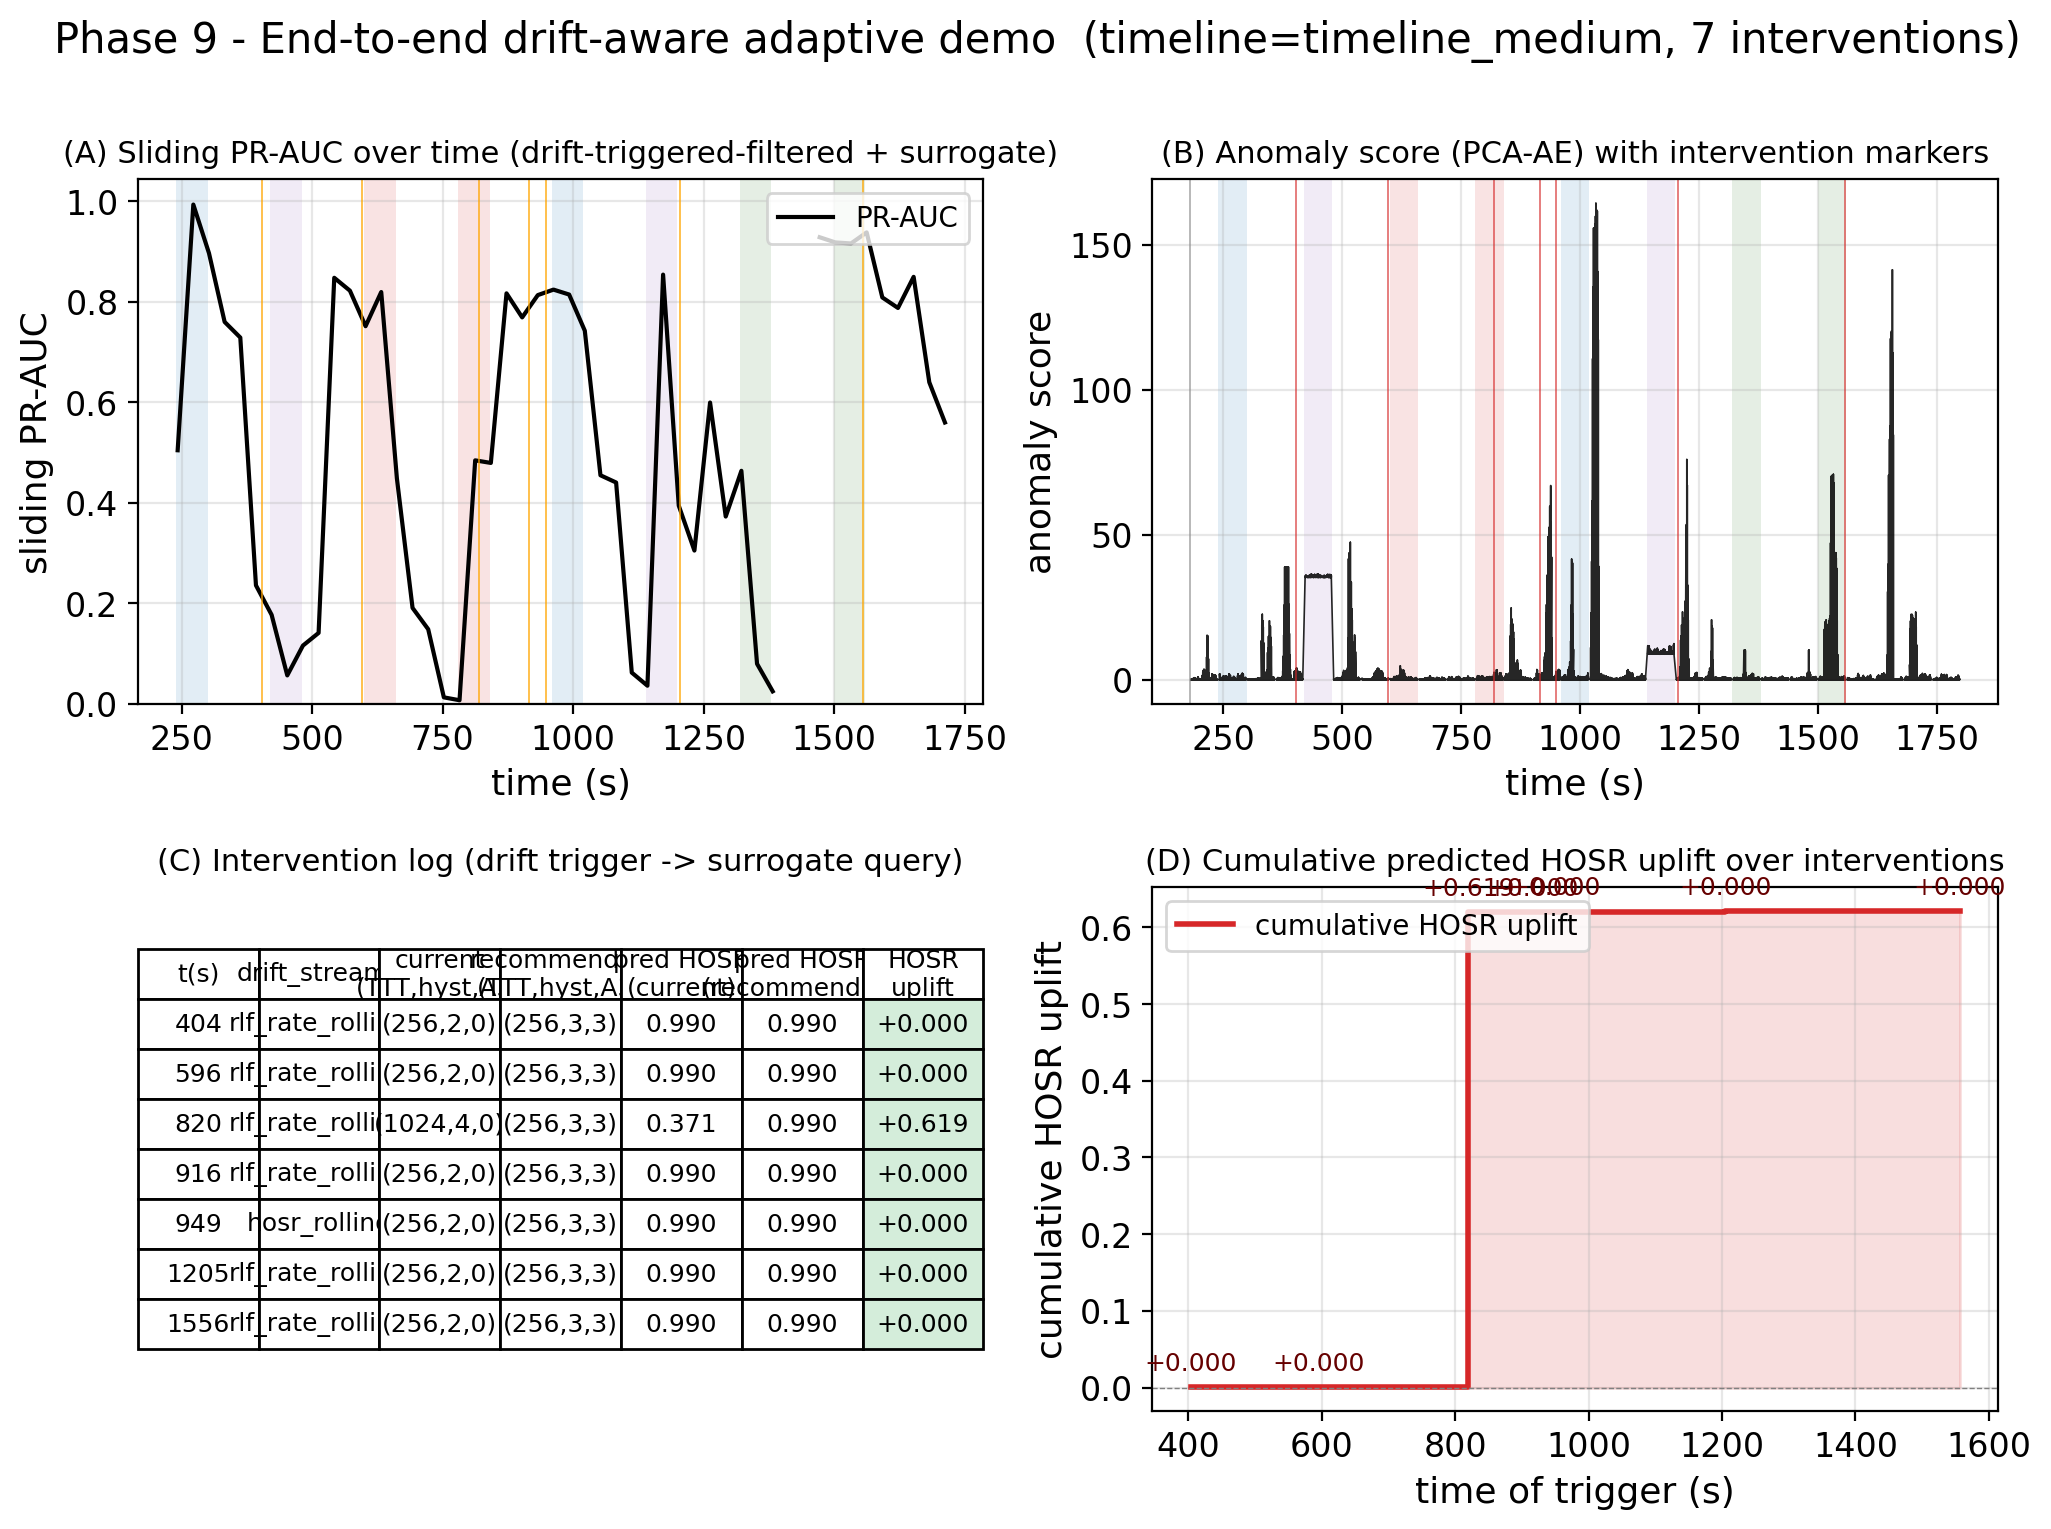
\includegraphics[width=.95\textwidth]{end_to_end_moneyshot}
\caption{End-to-end loop: sliding PR-AUC, anomaly score, interventions and cumulative HOSR uplift (own elaboration).}
\label{fig:end2end}
\end{figure}

\section{External validation}
\label{sec:res-external}

How far do these results travel? Table~\ref{tab:external} summarises the three
checks. First, a cross-seed replication over five master
seeds: the drift-volume is stable (coefficient of variation $0.04$), the
filtered-beats-naive gap replicates ($+0.072$, 95\% CI $[+0.033, +0.113]$), the
end-to-end HOSR uplift is essentially identical across seeds
($+0.621$), and the pooled anomaly winner is Isolation Forest in all five seeds.
The one criterion that does not pass is the stability of the \emph{per-type}
anomaly winner, which alternates between LOF, One-Class SVM and MLP-AE across
seeds; this is consistent with the tight per-type cluster seen in
Section~\ref{sec:res-anomaly} and is reported transparently as a limitation.

Second, a cross-scenario check on a denser urban timeline: all five criteria
pass. The filtered-beats-naive sign is preserved, and the end-to-end uplift not
only holds but scales to $+1.24$, consistent with there being more to gain when
mobility is more demanding. Third, a face-validity check on real NordicDat
5G-NSA telemetry, run fully self-supervised: the monitor flags only $1.2\%$ of
windows (well under the $10\%$ sanity ceiling) and its flagging peaks at the
$13{:}00$ commute hour ($3.5\times$ the daily mean), which is operationally
plausible. Because that data has no ground truth, no precision or recall is
claimed.

\begin{table}[ht]
\centering
\caption{External-validation headline outcomes (own elaboration).}
\label{tab:external}
\begin{tabular}{@{}lll@{}}
\toprule
Check & Result & Verdict \\
\midrule
Cross-seed: filtered $>$ naive      & $+0.072$ [$+0.033,+0.113$] & pass \\
Cross-seed: end-to-end HOSR uplift  & $+0.621$ (CV $\approx 0$)  & pass \\
Cross-seed: per-type anomaly winner & unstable (LOF/OCSVM/MLP-AE) & fail \\
Cross-scenario (dense urban)        & all 5 criteria; uplift $+1.24$ & pass \\
NordicDat face validity             & $1.2\%$ flagged, $13{:}00$ peak & pass \\
\bottomrule
\end{tabular}
\end{table}

\section{Discussion}
\label{sec:res-discussion}

Taken together, the four layers are consistent with the thesis premise that
handover monitoring benefits from being anomaly- and drift-aware rather than
trained once and left unchanged. Anomaly detection works well for structured
faults but struggles with subtle, single-UE or short cell-local ones, which sets
a realistic expectation for what an unsupervised monitor can catch. Drift
detection is dependable but involves an explicit latency-versus-false-alarm
choice. The adaptive layer suggests that retraining after drift can make things
worse if applied naively, and that a simple self-supervised filter is what allows
retraining to yield a net gain. Finally, the surrogate links configuration to
outcome accurately enough to suggest a recovery configuration after a harmful
change, with calibrated uncertainty. The main
limitations follow directly from the design: the anomalies are injected rather
than observed in the field, the KPI uplift is a surrogate prediction rather than
a measured gain, and the per-type anomaly ranking is seed-sensitive. These are
revisited as future work in the next chapter.


% !TEX encoding = UTF-8 Unicode
% !TEX root = thesis.tex

\chapter*{Summary and Conclusions}

This thesis investigated machine-learning-based, drift-aware monitoring for
handover (HO) optimization in 5G/6G radio access networks. Because no public
5G-SA dataset exposes both the HO control parameters and the resulting mobility
KPIs, the main data was produced with a custom, 3GPP-compliant 5G NR SA
handover simulator; its radio layer was calibrated against the real NordicDat
drive-test dataset and additionally checked through an external face-validity
test, with the real data never merged into the simulated benchmark. Returning to
the aim and the four research questions:

\begin{itemize}
  \item \textbf{RQ1 (anomaly detection):} unsupervised detectors catch
  structured faults well (measurement-glitch PR-AUC up to $0.858$, RLF-burst up
  to $0.751$) but subtle faults (interference spikes and slow single-UE
  degradation) stay near the noise floor; pooled over the timeline Isolation
  Forest is the strongest single detector (PR-AUC $0.425$), and an ablation shows
  the RSRQ feature family is the most informative by a wide margin.
  \item \textbf{RQ2 (drift):} every injected drift is detected by every detector
  (no misses), so the practical question is a latency-versus-false-alarm
  trade-off---batch two-sample tests (Energy/MMD) fire in $\approx 3$\,s at a
  high false-alarm rate, whereas sequential detectors (ADWIN/DDM) keep false
  alarms near $0.005$ per second but react more slowly.
  \item \textbf{RQ3 (adaptation):} the central result, and a somewhat surprising one,
  is that \emph{how} a monitor is retrained matters more than \emph{whether} it
  is retrained. Naive periodic or drift-triggered refits roughly halve PR-AUC
  ($0.264 \rightarrow \approx 0.12$) through self-poisoning, whereas a
  self-supervised filtered refit preserves the static baseline overall
  ($0.248$ vs $0.264$) and more than triples drift-phase PR-AUC
  ($0.057 \rightarrow 0.187$), at lower cost.
  \item \textbf{RQ4 (performance impact and reconfiguration):} a
  gradient-boosting configuration--performance surrogate predicts mobility KPIs
  accurately (HOSR $R^2 = 0.96$, RLF $R^2 = 0.95$, ping-pong $R^2 = 0.72$) with
  split-conformal intervals that restore calibrated coverage; an inverse query
  returns $12$ of $36$ feasible configurations (favouring the shortest
  time-to-trigger), and an end-to-end detect--recommend--recover loop fires seven
  interventions for a cumulative, model-predicted HOSR uplift of $+0.62$.
\end{itemize}

\section*{Limitations}

The scope is 5G NR SA intra-RAT inter-gNB Xn handover; NSA, intra-gNB and
inter-RAT mobility are out of scope. The framework is deliberately positioned as
monitoring and decision support rather than as a parameter-tuning control loop:
automatic tuning of time-to-trigger, hysteresis and cell individual offset is
already standardized as mobility robustness optimization (MRO)~\cite{tr36839,ts28313},
and the reconfiguration step here is intended to feed such a function rather than
to replace it. In contrast to MRO, which acts on lagging mobility-failure
counters, the system intervenes on leading drift indicators; it does not,
however, forecast the failure of an individual handover before it occurs. The
anomalies are \emph{injected} in
simulation rather than observed in the field; the reported HOSR uplift is a
surrogate \emph{model prediction}, not a measured field gain; the RSRQ radio
layer retains a residual calibration mismatch (KS $0.467$); and the
per-anomaly-type best detector is seed-sensitive, although the pooled detector
ranking and the filtered-over-naive result are stable across seeds and scenarios.

\section*{Future work}

Several concrete directions follow from the limitations above. The most immediate
is to bring the experimental environment closer to reality without relying on
operator event logs, which are rarely accessible in practice. This means richer
system-level simulators (for example ns-3 5G-LENA or Simu5G) and, longer term,
digital-twin style environments, while keeping the controlled injection of drift
and anomalies that makes labelled benchmarking possible; public drive-test
datasets such as NordicDat and the urban Bangladesh LTE handover set can continue
to serve as external face-validity references.

A second direction is continual (online, incremental) learning, so that the
anomaly monitor and the configuration-performance surrogate are updated
continuously under persistent change rather than refitted in batches. The
self-supervised filtering rule introduced here is a natural starting point and
should be made adaptive and given stability guarantees. A third direction is
explainability: identifying which KPIs, radio conditions, or parameter changes
are most strongly associated with handover degradation, so that a recommended
reconfiguration can be justified rather than only predicted. A related direction
is to move from detection toward genuine \emph{proactive} prediction: the present
framework reacts to the onset of drift on leading KPI streams, but it does not
forecast the failure of an individual handover before it happens. Adding an
event-level predictor (for example a per-UE time-to-failure or
handover-failure model that estimates the probability of a too-late or too-early
handover ahead of time) was kept out of the present scope because it requires
per-event prediction targets and a forecasting setup distinct from the
unsupervised monitoring studied here; combined with the configuration--performance
surrogate, such a predictor would let the system act before the precursor drift
fully materialises and connects naturally to the proactive handover-prediction
line of work reviewed in Section~\ref{subsec:rw-prediction}. Finally, the
configuration scope can be broadened beyond time-to-trigger, hysteresis, and A3
offset to include cell individual offset (CIO), and beyond intra-RAT inter-gNB to
the cases excluded here, moving toward a safe and interpretable decision-support
mechanism that limits unnecessary optimisation actions. Together these steps
extend handover monitoring toward the broader goal of drift-aware, explainable,
and adaptive mobility management.


% Bibliography
\bibliographystyle{dyplom}
\bibliography{bibliography}

% Lists of figures and tables
\listoffigures
\listoftables

% Appendices - comment out if not applicable
\appendixpage
\appendix
% !TEX encoding = UTF-8 Unicode
% !TEX root = thesis.tex
%
% AI-tools usage disclosure, required by the Faculty (WIT PWr) GenAI guidelines.
% Agree the exact wording and scope with your supervisor before submission.

\chapter{Declaration on the Use of AI Tools}
\label{app:ai}

In accordance with the Faculty of Information and Communication Technology
guidelines on the use of generative AI tools and the University's seven
recommendations, the use of AI tools in this thesis is disclosed below.

\begin{itemize}
  \item \textbf{Tool(s) used:} Anthropic Claude, used through the Cursor IDE.
  \item \textbf{Purpose and scope:} the tool was used for language editing and
  proofreading, for drafting and structuring parts of the LaTeX document, and as
  a supporting tool for code drafting while building the simulator and the
  data and analysis pipeline and figures.
  \item \textbf{What was \emph{not} delegated to AI:} the research design, the
  choice of methods and scenarios, the interpretation of the results, and the
  conclusions are the author's own.
  \item \textbf{Verification:} all AI-assisted content (text, code, references)
  was reviewed and verified by the author, who takes full responsibility for it.
\end{itemize}

% Note: confirm with your supervisor whether a prompt/response log is required.


\end{document}
